\documentclass[11pt]{my_memo}
\usepackage{longtable,booktabs,array}
\usepackage{graphicx}
\usepackage[hyphens]{url}
% a case name may break after an underscore or a slash
\newcommand{\case}[1]{\seqsplit{#1}}
\usepackage{seqsplit}
% The text block is the class default; the wide tables are set one font size
% down so that a case name still stands on one line.
\setlength{\tabcolsep}{3pt}
\renewcommand{\arraystretch}{1.0}
\title{The LHS 1140 b catalog: what is certified and what is not}
\author{EXHALE}
\date{2026-09-29}
\begin{document}
\maketitle

\begin{center}
\fbox{\parbox{0.92\textwidth}{\textbf{Two physics in this summary.} Section~5
(the molecular $K_{zz}=10^{9}$ family) was rewritten on 2026-09-26 from
states certified under the atomic data as corrected on 2026-09-24 to
2026-09-26 (\texttt{md/Update\_EXHALE\_stage3.md} sections 17 to 27). Every
other state, equivalent width, crossing and certificate below is of the
physics before those corrections: none of those certificates holds under the
corrected physics, and their equivalent widths are not current (the molecular
family's crossing moved from He/H~=~1.46 to 1.70 on the catalog grid).
\textbf{The code moved again on 2026-09-26 to 2026-09-28} (sections 29.1 to
29.12 of the same log: an OpenMP race in the metal sweep, the interdiffusion
enthalpy flux, the He$^+$\,+\,H charge exchange near threshold, the
\texttt{\_adv} post-process made second order, the lower face placed at the
reservoir level): every number of this summary, section~5 included,
predates those changes. \textbf{On 2026-09-29 the code moved once more}
(sections 33 to 37): the sensible enthalpy the transported molecular
carriers carry is in the energy equation (default on), and under
\texttt{Well balanced: True} the base boundary shares the reconstruction's
discrete hydrostatic equilibrium (boundary model
\texttt{\ldots\_discrete\_equilibrium\_v5}), which removes a base mass flux of
up to $10^{4}$ times a weak wind. Two continuation states certified under
the previous boundary re-certified under it in 2 and 4 passes (MEASURED).
By the user's decision of 2026-09-26 certified rows are not re-solved after
each change; the models that did not solve come first (section~3).}}
\end{center}

\noindent
Every model of the catalog is LHS 1140 b on 500 cells, solved by the
partitioned stationary route with \texttt{Well balanced: True}, from the
GJ~1132 spectrum placed at this planet's orbit. The binary of record of the
rows solved up to 2026-09-22 is \texttt{EXHALE\_75d55d9d.x}, md5
\texttt{75d55d9d4fd0e748cd01d6e35713e34c}; the rows added on 2026-09-23 and
2026-09-24 were solved and certified under \texttt{EXHALE\_69233669.x} (the
He/H~=~9.7 rungs below 0.07 of the fiducial XUV) and
\texttt{EXHALE\_46d5b9f4.x} (the molecular $K_{zz}=10^{9}$ rungs), as the
table notes say. Five molecular $K_{zz}=10^{9}$ rows were certified after
the atomic-data corrections began: He/H~=~1.45 on 2026-09-25 under
\texttt{EXHALE\_b059a4be.x} (the second of five rounds of corrections), and
1.52, 1.6, 1.8 and 2.13 on 2026-09-26 under the binary of record,
\texttt{EXHALE\_7db5afe9.x}, md5 \texttt{7db5afe9b1d80ce757fcc07d1b499330}
(section~5). Three molecular rows were published on 2026-09-29 from states
the continuation of \texttt{md/Update\_EXHALE\_stage3.md} sections 29.13,
34 and 37 certified: the photochemical \case{photochem\_kzzprofile/HeH9} and
\case{photochem\_kzzprofile/HeH2.09} under \texttt{EXHALE\_6dd54955.x}
(base boundary model v4, with the enthalpy flux of the transported
carriers) and \case{scalar\_wellmixed/HeH0.55} under
\texttt{EXHALE\_3c22c63e.x} (the discrete-equilibrium boundary model v5),
as the table notes of section~4 say. The counts below are MEASURED by
\texttt{models/status.py inventory}, re-run read-only on 2026-09-29, which
names \texttt{EXHALE\_6dd54955.x}, md5
\texttt{6dd549556910351a7f857708b4853a69}, as the binary of record:
\textbf{210 state indexes, 155 certified} (158 and 103 earlier on
2026-09-29, before the continuation rungs were published; 157 and 100 on
2026-09-24 and 2026-09-26; 143 and 92 on 2026-09-22). These counts are of
the recorded certificates: the molecular rows published on 2026-09-29 were
measured under the binaries their table notes name (section~4), all other
rows under binaries before the atomic-data corrections. A case
counts as certified when its index names a \texttt{latest\_certified}
generation that no refused re-evaluation has marked stale. Section 3 and
section 4 list the 156 models of the ladders and of \texttt{diffusion\_check};
the remaining 54 indexes are 46 flux-closure iterates, two archival copies,
one study directory and five run directories the low-XUV rungs left.
Section~5, rewritten on 2026-09-26 under the corrected atomic physics: the
molecular $K_{zz}=10^{9}$ family straddles the observed equivalent width
with two certified rungs (He/H~=~1.6 and 1.8), the crossing moves with the
grid to about 1.84 in the continuum limit, and the added Gaussian those
solutions need to reproduce the width of the measured line is recorded.

\paragraph{Where each column comes from.} $du$ and $\lVert R\rVert$ are
both read from the LAST \texttt{(JFNK) done} line of the case's
\texttt{run.log}, so they are one pair printed by one solve and not two
numbers from two places; where a case was last re-measured by an evaluation
that took no step, that line is the solve preceding it, and where a case was
never advanced there is none and the columns read \texttt{--}. The refusing
rows of section 3 are read from \texttt{certification.txt} of the generation
the case's index names \texttt{latest\_complete}, and EVERY refusing entry of
that certificate is listed, not only the first. $\log_{10}\dot{M}$ and the
equivalent width are from \texttt{models/status.py}, which reads them from
the case directory. The equivalent width is the red-pair integral over the
vacuum window 10832.60 to 10834.20~\AA\ taken on the observation's own
wavelength samples: the instrument-convolved model is interpolated onto the 44
samples of the measurement inside the window and integrated with their
trapezoid weights, the same operator that gives the observed
$1.108$~\%\,\AA\ (\texttt{LHS1140b/he10830\_equivalent\_width.py}, adopted
2026-09-23). Integrated on its own finer grid instead, a model differs by at
most $1.5\times10^{-4}$~\%\,\AA\ over the catalog, which moves 15 of the
91 certified rows below in the fourth decimal (MEASURED 2026-09-24). The XUV column is the factor the stellar spectrum is scaled
by; $K_{zz}$ is the eddy coefficient of the base, \emph{profile} where a
photochemical column supplies $K_{zz}(p)$, and \emph{none} where the base is
well mixed. The \emph{wind chemistry} column of every table below says what
is solved ABOVE the base, atomic or molecular in the sense of section 1; what
supplies the base itself is in the case name (\texttt{scalar} or
\texttt{photochem}) and in the $K_{zz}$ column.

\section{Two axes: where the lower atmosphere comes from, and what the wind solves}

A case name carries both axes, and they are independent. The first says what
supplies the state at the base level, the second whether the wind above it
carries a molecular network at all.

\paragraph{The lower boundary.}
\begin{itemize}
\item \texttt{scalar}: the base is a few prescribed numbers at the level,
      read from \texttt{base.inp}: the pressure (1 microbar), the temperature
      (226 K), the base radius, the bound hydrogen fraction $q_{\rm H2,base}$
      and the element reservoirs. Nothing below the level is modeled.
\item \texttt{scalarCNO}: the same scalar base with the C, N and O reservoirs
      of the photochemical column added at the matching level.
\item \texttt{photochem}: the lower atmosphere is a Photochem column handed
      over as a PROFILE, the key \texttt{Lower atmosphere profile:} naming a
      file \texttt{lower\_atmosphere\_profile.dat}, which carries $T(p)$, $K_{zz}(p)$, the
      bound hydrogen fraction and the element reservoirs at the matching
      level $p_{\rm match} = 1$ microbar. For the atomic groups the reservoir
      He/H is then solved by the elemental-flux closure
      (\texttt{src/utils/element\_flux\_closure.py}), which iterates the
      column and the wind against each other: the iterates are the
      \texttt{k<NN>} directories, and the composition is an output of that
      loop rather than an input.
\end{itemize}

\paragraph{The wind's chemistry.}
\begin{itemize}
\item \texttt{atomic}: hydrogen and helium with their ionization stages and,
      where the group says so, trace metals. No molecular network is solved
      above the base, whatever the base carries.
\item \texttt{molecular}: EXHALE's own network, \texttt{Molecular chemistry:
      True} with \texttt{Molecular carrier transport: True}, solving H$_2$,
      H$_2^+$, H$_3^+$ and HeH$^+$ in the wind with the H$_2$ carrier
      transported. The molecular base it starts from is the scalar handoff or
      the profile, by the other axis.
\end{itemize}

\noindent
So \texttt{atomic\_photochem\_...} is a Photochem column under an atomic
wind, and \texttt{molecular\_scalar\_...} is EXHALE's own molecular chemistry
above a scalar base. The two are not alternatives for the same layer: the
Photochem column is the atmosphere BELOW the matching level, and EXHALE's
network is the chemistry ABOVE it. A \texttt{molecular\_photochem} case uses
both, the column below and the network above.

\begin{center}
\footnotesize
\begin{tabular}{@{}l l l@{}}
\toprule
 & wind solved atomic & wind solved with EXHALE's molecular network\\
\midrule
scalar base (\texttt{base.inp}) & \texttt{atomic\_scalar\_*} & \texttt{molecular\_scalar\_*}\\
Photochem column (profile) & \texttt{atomic\_photochem\_*} & \texttt{molecular\_photochem\_*}\\
\bottomrule
\end{tabular}
\end{center}

\noindent
The mixing suffix is a third, smaller axis: \texttt{wellmixed} is no element
diffusion, \texttt{kzz1e9} is binary H/He diffusion at that eddy coefficient,
and \texttt{kzzprofile} takes $K_{zz}(p)$ from the column.

\section{By group}

\scriptsize\linespread{1.0}\selectfont\begin{longtable}{@{}l >{\raggedright\arraybackslash}p{1.5cm} >{\raggedright\arraybackslash}p{1.9cm} l l l l r r@{}}
\toprule
group & wind chemistry & He/H & XUV & $K_{zz}$ & diff. & $du$ reached & cases & cert.\\
\midrule
\endhead
\case{diffusion\_check} & atomic & 0.55 & 1 & 0.0 to 1.0e9 & on & -- & 4 & 0\\
\case{photochem\_x0.01\_kzzprofile} & atomic & 9.7 & 0.01 & profile & on & 9.4E-03 & 1 & 0\\
\case{photochem\_x0.10\_kzzprofile} & atomic & 9.7 & 0.10 & profile & on & 5.0E-10 & 1 & 1\\
\case{photochem\_x0.15\_kzzprofile} & atomic & 9.7 & 0.15 & profile & on & 4.7E-12 & 1 & 1\\
\case{photochem\_x0.20\_kzzprofile} & atomic & 9.7 & 0.20 & profile & on & 2.0E-12 & 1 & 1\\
\case{photochem\_x0.25\_kzzprofile} & atomic & 9.7 & 0.25 & profile & on & 1.9E-12 & 1 & 1\\
\case{photochem\_x0.30\_kzzprofile} & atomic & 9.7 & 0.30 & profile & on & 1.3E-10 & 1 & 1\\
\case{photochem\_x0.33\_kzzprofile} & atomic & 9.7 & 0.33 & profile & on & 1.6E-10 & 1 & 1\\
\case{scalarCNO\_kzz1e9} & atomic & 2.13 & 1 & 1.0e9 & on & 1.7E-11 & 1 & 1\\
\case{scalar\_gj699\_wellmixed} & atomic & 0.042 to 1000 & 1 & none & off & 1.8E-13 to 1.6E-11 & 6 & 6\\
\case{scalar\_kzz0} & atomic & 0.55 to 3.9 & 1 & 0.0 & on & 2.4E-11 to 1.2E-10 & 6 & 6\\
\case{scalar\_kzz1e10} & atomic & 0.55 to 1.29 & 1 & 1.0e10 & on & 2.0E-11 to 2.7E-11 & 4 & 4\\
\case{scalar\_kzz1e11} & atomic & 0.55 to 0.93 & 1 & 1.0e11 & on & 1.8E-11 to 1.9E-10 & 4 & 4\\
\case{scalar\_kzz1e5} & atomic & 2.6 to 3.93 & 1 & 1.0e5 & on & 2.5E-11 to 4.8E-11 & 5 & 5\\
\case{scalar\_kzz1e6} & atomic & 0.55 to 3.74 & 1 & 1.0e6 & on & 1.9E-11 to 6.8E-11 & 6 & 6\\
\case{scalar\_kzz1e7} & atomic & 0.55 to 3.18 & 1 & 1.0e7 & on & 1.6E-12 to 1.3E-10 & 4 & 4\\
\case{scalar\_kzz1e8} & atomic & 0.55 to 2.41 & 1 & 1.0e8 & on & 5.5E-11 to 7.9E-11 & 4 & 4\\
\case{scalar\_kzz1e9} & atomic & 0.55 to 9.7 & 1 & 1.0e9 & on & 9.3E-13 to 6.1E-11 & 7 & 7\\
\case{scalar\_wellmixed} & atomic & 0.083 to 1000 & 1 & none & off & 1.4E-12 to 1.2E-10 & 9 & 9\\
\case{scalar\_x0.015\_kzz1e9} & atomic & 2.13 & 0.015 & 1.0e9 & on & 1.8E-10 & 1 & 1\\
\case{scalar\_x0.01\_kzz1e9} & atomic & 2.13, 9.7 & 0.01 & 1.0e9 & on & 4.4E-12 to 2.2E-10 & 2 & 1\\
\case{scalar\_x0.02\_kzz1e9} & atomic & 2.13 & 0.02 & 1.0e9 & on & 8.3E-11 & 1 & 1\\
\case{scalar\_x0.03\_kzz1e9} & atomic & 2.13 & 0.03 & 1.0e9 & on & 4.4E-11 & 1 & 1\\
\case{scalar\_x0.05\_kzz1e9} & atomic & 2.13 & 0.05 & 1.0e9 & on & 6.4E-11 & 1 & 1\\
\case{scalar\_x0.06\_kzz1e9} & atomic & 9.7 & 0.06 & 1.0e9 & on & 2.8E-12 & 1 & 0\\
\case{scalar\_x0.0624\_kzz1e9} & atomic & 9.7 & 0.0624 & 1.0e9 & on & 3.1E-12 & 1 & 0\\
\case{scalar\_x0.065\_kzz1e9} & atomic & 9.7 & 0.065 & 1.0e9 & on & 2.6E-12 & 1 & 1\\
\case{scalar\_x0.0662\_kzz1e9} & atomic & 9.7 & 0.0662 & 1.0e9 & on & 2.5E-12 & 1 & 1\\
\case{scalar\_x0.0675\_kzz1e9} & atomic & 9.7 & 0.0675 & 1.0e9 & on & 3.3E-12 & 1 & 1\\
\case{scalar\_x0.07\_kzz1e9} & atomic & 2.13, 9.7 & 0.07 & 1.0e9 & on & 7.0E-12 to 5.1E-11 & 2 & 2\\
\case{scalar\_x0.10\_kzz1e9} & atomic & 2.13, 9.7 & 0.10 & 1.0e9 & on & 4.4E-12 to 1.5E-11 & 2 & 2\\
\case{scalar\_x0.15\_kzz1e9} & atomic & 2.13, 9.7 & 0.15 & 1.0e9 & on & 8.2E-12 to 9.1E-12 & 2 & 2\\
\case{scalar\_x0.20\_kzz1e9} & atomic & 2.13, 9.7 & 0.20 & 1.0e9 & on & 5.5E-12 to 1.1E-11 & 2 & 2\\
\case{scalar\_x0.25\_kzz1e9} & atomic & 2.13, 9.7 & 0.25 & 1.0e9 & on & 5.2E-12 to 1.7E-11 & 2 & 2\\
\case{scalar\_x0.30\_kzz1e9} & atomic & 2.13, 9.7 & 0.30 & 1.0e9 & on & 3.2E-12 to 5.6E-12 & 2 & 2\\
\case{scalar\_x0.33\_kzz1e9} & atomic & 2.13, 9.7 & 0.33 & 1.0e9 & on & 2.8E-12 to 3.4E-12 & 2 & 2\\
\case{photochem\_kzzprofile} & molecular & 2.09, 9 & 1 & profile & on & 3.6E-12 to 4.9E-12 & 2 & 2\\
\case{scalar\_kzz1e9} & molecular & 0.083 to 9.7 & 1 & 1.0e9 & on & 8.2E-13 to 1.2E-10 & 40 & 39\\
\case{scalar\_wellmixed} & molecular & 0.083 to 2.13 & 1 & none & off & 7.8E-13 to 2.5E-10 & 22 & 21\\
\midrule
\multicolumn{7}{l}{total} & 156 & 146\\
\bottomrule
\end{longtable}\normalsize

\noindent
Besides these, the catalog holds 46 flux-closure iterates \texttt{k<NN>},
two archival copies, one study directory and five run directories of the
low-XUV rungs (each run keeps the case files it ended with, and its index
counts in the inventory). Nine of the iterates carry a
certificate; the other 37 were written by runs that asked for no time
integration, so they are states that were post-processed and never advanced,
and they are not failures of a solve.

One molecular case carries no index at all and is not counted in the table:
\case{molecular\_scalar\_gj1132\_wellmixed/HeH2.13} was attempted and
published no state (section~3). \case{molecular\_photochem\_gj1132\_kzzprofile/HeH2.09},
which was in the same position, has published a certified state since
2026-09-29 (section~4).

\section{The models that are not certified}

Ten of the 156 indexed models carry no certificate. Four of them, the
\texttt{diffusion\_check} rows, are not models of their own: each is the
post-processing pass of a certified case repeated with
\texttt{EXHALE\_DIFFUSION\_CHECK=1} (\texttt{Do only PP: True}, CFL
$10^{-12}$; \texttt{models/diffusion\_check/README.md}) to write the element
face-flux table, and it makes no stationary claim
(\texttt{cert\_reason=no\_stationary\_claim}). The four cases they repeat, the \texttt{HeH0.55} rungs of
\texttt{atomic\_scalar\_gj1132\_kzz0}, \texttt{\_kzz1e8}, \texttt{\_kzz1e9}
and \texttt{\_kzz1e10}, are certified (\texttt{certified\_in\_wind}, read 2026-09-29), and the rows the
certificate refuses on below are those of the post-processed state, not of a
solve. The other six were solved, or attempted, or written without being
advanced at all, and the certificate of the generation its index names
refuses them. The last column lists every entry of
that certificate that stands above its tolerance, with the measure and the
cell, in the certificate's own order.

\scriptsize\linespread{1.0}\selectfont\begin{longtable}{@{}l >{\raggedright\arraybackslash}p{1.1cm} l l l l l l >{\raggedright\arraybackslash}p{4.3cm}@{}}
\toprule
case & wind chemistry & He/H & XUV & $K_{zz}$ & diff. & $du$ & $\lVert R\rVert$ & the rows the certificate refuses on\\
\midrule
\endhead
\case{diffusion\_check/scalar\_kzz0\_HeH0.55} & atomic & 0.55 & 1 & 0.0 & on & -- & -- & mass 1.541 at cell 1; momentum 7.593e-3 at cell 500; energy 1.583 at cell 5; elemental He/H 2.546e-4 at cell 500\\
\case{diffusion\_check/scalar\_kzz1e10\_HeH0.55} & atomic & 0.55 & 1 & 1.0e10 & on & -- & -- & mass 1.541 at cell 1; momentum 2.466e-3 at cell 500; energy 1.907 at cell 5; elemental He/H 9.644e-5 at cell 500\\
\case{diffusion\_check/scalar\_kzz1e8\_HeH0.55} & atomic & 0.55 & 1 & 1.0e8 & on & -- & -- & mass 1.542 at cell 1; momentum 5.150e-3 at cell 500; energy 1.952 at cell 5; elemental He/H 1.790e-4 at cell 500\\
\case{diffusion\_check/scalar\_kzz1e9\_HeH0.55} & atomic & 0.55 & 1 & 1.0e9 & on & -- & -- & mass 1.542 at cell 1; momentum 3.719e-3 at cell 500; energy 1.917 at cell 5; elemental He/H 1.354e-4 at cell 500\\
\case{photochem\_x0.01\_kzzprofile/HeH9.7} & atomic & 9.7 & 0.01 & profile & on & 9.356E-03 & 1.163E+00 & mass 5.880e-1 at cell 11; momentum 7.774e-7 at cell 495; energy 1.949 at cell 7; elemental He/H 3.538e-2 at cell 389\\
\case{scalar\_x0.01\_kzz1e9/HeH9.7} & atomic & 9.7 & 0.01 & 1.0e9 & on & 4.424E-12 & 9.978E-01 & mass 9.806e-1 at cell 2; momentum 8.724e-6 at cell 1; energy 1.071 at cell 1\\
\case{scalar\_x0.06\_kzz1e9/HeH9.7} & atomic & 9.7 & 0.06 & 1.0e9 & on & 2.785E-12 & 5.589E-07 & elemental He/H 2.508e-2 at cell 333\\
\case{scalar\_x0.0624\_kzz1e9/HeH9.7} & atomic & 9.7 & 0.0624 & 1.0e9 & on & 3.086E-12 & 8.091E-08 & elemental He/H 1.435e-2 at cell 333\\
\case{scalar\_kzz1e9/HeH0.083} & molecular & 0.083 & 1 & 1.0e9 & on & 4.879E-12 & 1.369E-08 & H$_2$ carrier 8.150e-4 at cell 499; elemental He/H 2.503e-4 at cell 280\\
\case{scalar\_wellmixed/HeH0.083} & molecular & 0.083 & 1 & none & off & 6.592E-12 & 2.701E-08 & H$_2$ carrier 7.371e-2 at cell 500\\
\bottomrule
\end{longtable}\normalsize

\noindent
Read by mechanism, the ten fall into three kinds.
\begin{itemize}
\item \textbf{The four atomic He/H~=~9.7 models at 0.01 to 0.0624 of the
      fiducial XUV} (the hydrodynamic Newton made no progress at 0.01; the
      elemental He/H row refused 0.06 and 0.0624 at cell 333). Their catalog
      states lie on the grid before the lower face was placed at the level,
      so they load only as seeds mapped onto the present grid, and there the
      stationary solve fails on every pass (\texttt{info~=~2}). The mapped
      seeds are winds (mass-flux spread 0.3 per cent), but their lower
      layer is off the grid's discrete hydrostatic equilibrium by about
      $10^{-3}$ of the pressure, which the Roe pressure-jump term turns into
      a numerical mass flux of up to $10^{4}$ times the wind; projected onto
      that equilibrium (with the base boundary sharing it), the mass and
      momentum rows fall from 1.9 and $5\times10^{-3}$ to
      $3.7\times10^{-3}$ and $8\times10^{-7}$ on the 0.06 seed, and the energy
      row, about 1, is what remains: the heat of the base cell and the
      interdiffusion enthalpy flux of a composition that is not in its
      diffusive steady state near the base. Stationary solves from the
      projected seeds are running
      (\texttt{md/atomic\_heh97\_reduced\_xuv\_20260929.md}, its review, and
      \texttt{md/Update\_EXHALE\_stage3.md} sections 35 to 37).
\item \textbf{The composition half of the solve refuses} the two
      molecular models: the H$_2$ carrier balance in both, and in
      \case{scalar\_kzz1e9/HeH0.083} also the elemental He/H row. The wind
      itself is converged in both. The next subsection says what was
      measured. Two more molecular models stood in this table until
      2026-09-29, \case{photochem\_kzzprofile/HeH9} and
      \case{scalar\_wellmixed/HeH0.55}; they were reached by continuation and
      their certified states are published (section~4). The two that remain
      are approached to He/H~=~0.19 and 0.1 (the subsection after next).
\item \textbf{Nothing was solved} in the four \texttt{diffusion\_check}
      rows: they are post-processing passes of four certified cases, made
      without a time integration, so they have no $du$ and no
      $\lVert R\rVert$. Their certificates were measured all the same, and
      refuse on the hydrodynamic rows and the elemental row, which is what an
      unadvanced state is expected to do; they are not failures of a solve,
      and not models of their own.
\end{itemize}

\paragraph{What the two numbers say.} $du$ is the fractional spread of the
mass flux $\rho v r^2$ over the wind window, the quantity a marching run stops
on, and $\lVert R\rVert$ is the stationary operator's residual norm. The
recipe of this code, and the practice of the literature it follows, calls a
wind converged at $du < 10^{-3}$. MEASURED on the models that carry no
certificate, naming the wind chemistry because the same short name occurs in
both families: the molecular \case{scalar\_kzz1e9/HeH0.083} reaches
$du = 4.9\times10^{-12}$ with $\lVert R\rVert = 1.4\times10^{-8}$, the
molecular \case{scalar\_wellmixed/HeH0.083} $6.6\times10^{-12}$ and
$2.7\times10^{-8}$, and the atomic
\case{scalar\_x0.01\_kzz1e9/HeH9.7} $4.4\times10^{-12}$ with
$\lVert R\rVert = 1.0$, and the atomic He/H~=~9.7 rungs at 0.06 and 0.0624
$2.8\times10^{-12}$ and $3.1\times10^{-12}$ with $5.6\times10^{-7}$ and
$8.1\times10^{-8}$. By the flux-spread criterion these are converged winds,
and two of them also sit at a residual norm of $10^{-8}$.

What refuses them is this code's own row-by-row certification, which is
stricter: it measures every equation of the inventory cell by cell and names
each one that stands above its tolerance. Over the ten the elemental
He/H row appears in eight of them, the hydrodynamic energy, mass and
momentum rows in six each and the H$_2$ carrier balance in the
wind in two (MEASURED on the table above). A state that meets the flux-spread
criterion and fails one such row is a meaningful solution by the standard
other work uses, and the table says which rows keep it from this one.

\subsection*{Why the molecular winds do not certify}

\paragraph{The verdict.} The failure is of the method, not a finding that
these winds have no stationary state. The partitioned route alternates two
solves in every outer pass: the hydrodynamic Newton solve at fixed
composition, then the relaxation of the composition (the element rows and
the H$_2$ carrier) at fixed wind. For the six molecular cases below the
alternation does not approach a joint fixed point. The one route that
solves both halves together fails in its linear solve. Every measurement
of this subsection was made under binaries before the atomic-data
corrections, among them \texttt{EXHALE\_3146d11b.x} (2026-09-18) and the
tree's binary of 2026-09-21 (md5 \texttt{89ec6714...}). Whether the same
cases behave the same way under \texttt{EXHALE\_7db5afe9.x} was not
measured.

\paragraph{The six cases.} The two molecular rows of the table above, the
two that stood in it until they certified by continuation
(\case{photochem\_kzzprofile/HeH9} and \case{scalar\_wellmixed/HeH0.55},
section~4), and the two that published no index when these measurements
were made (READ from each case's \texttt{not\_solved.md}, now
\texttt{not\_solved\_<date>.md} where the case has solved since, and from
\texttt{md/lhs1140b\_stationary\_L34c\_20260918.md}); of those two,
\case{photochem\_kzzprofile/HeH2.09} has certified by continuation as well.
The two with no index were started from the certified atomic wind of the
same composition. Each was stopped at the six-hour ceiling:
\begin{itemize}
\item \case{molecular\_scalar\_gj1132\_wellmixed/HeH2.13}: the carrier H$_2$
      row flattened at $4.3\times10^{-1}$ after seven outer passes.
\item \case{molecular\_photochem\_gj1132\_kzzprofile/HeH2.09}: the row
      banded between 0.19 and 0.44 over twelve outer passes without a trend.
\end{itemize}

\paragraph{What six outer passes showed, measured on 2026-09-21.} Each of
four cases was advanced six outer passes from its stored state
(\texttt{md/lhs1140b\_alternation\_audit\_20260921.md}). Three did not
approach a fixed point, by two different mechanisms, and one did:
\begin{itemize}
\item \textbf{The composition update takes the wind out of solution}
      (\case{wellmixed/HeH0.083} and \case{wellmixed/HeH0.55}).
      \begin{itemize}
      \item One bounded composition update moved the mass flux by 0.985 of
            its own column scale.
      \item From pass 2 on, the hydrodynamic solve returned
            \texttt{info~=~2}, with its mass and energy rows seven decades
            above tolerance, and never recovered.
      \item In \case{wellmixed/HeH0.55} the H$_2$ front also walked outward:
            the refusing cell moved from 306 to 349 ($r = 1.95$ to
            3.02~$R_p$) while the row rose by a factor 4.5.
      \end{itemize}
\item \textbf{A drift under a saturated movement bound}
      (\case{kzz1e9/HeH0.083}).
      \begin{itemize}
      \item The carrier relaxation ended on its movement bound in every pass,
            at cells 418 to 426 ($r = 8.0$ to 8.7~$R_p$).
      \item The gated carrier row rose from $8.2\times10^{-4}$ to
            $2.9\times10^{-3}$, while the hydrodynamic rows stayed within
            tolerance.
      \item Relocating the bound does not help: the bound then acts at the
            edge of the mask, and the refusing row rises in every such run
            (2026-09-17). So the bound is not the defect.
      \end{itemize}
\item \textbf{Approaching, and stopped by the budget}
      (\case{kzz1e9/HeH0.55}): the joint residual fell 3.7 decades in five
      passes. This case was then finished and certified on 2026-09-24
      (section~4).
\end{itemize}

\paragraph{The route that solves both halves together fails.} Two
measurements show it, on 2026-09-17 and 2026-09-21
(\texttt{md/lhs1140b\_coupled\_trial\_20260921.md}). With
\texttt{Coupled carrier solve: True}, the element and H$_2$ carrier rows
become unknowns of the Newton solve.
\begin{itemize}
\item On \case{kzz1e9/HeH0.083}, that solve spent 41 trust-region
      iterations, 6632 residual evaluations and 7172~s. It moved the merit
      only from $9.720\times10^{-2}$ to $9.718\times10^{-2}$, stagnated
      (\texttt{info~=~2}) and handed back the state it started from.
\item On a case the alternation certifies, all 13 linear solves exhausted
      their 40-vector Krylov subspace at a relative residual of 0.26 against
      the 0.1 asked.
\end{itemize}
The missing piece is a preconditioner that holds the species rows. It is
the open item that owns these cases.

\paragraph{Explanations excluded by measurement.} These are, in order:
\begin{itemize}
\item \emph{An outer boundary that traps H$_2$.} At cell 500 the diffusive
      face is exactly zero, because the carrier's ghost repeats the last
      value. Opening that face makes the refusing row worse, by factors 1.12
      to 182: H$_2$ is heavier than the mean particle of the ionized wind,
      so the settling drift the open face admits points inward.
\item \emph{An inexact inner solve.} In each pass the element relaxation
      reached the fixed point of its own operator.
\item \emph{A two-state cycle.} The two-pass state difference is never small
      against the one-pass differences it spans.
\item \emph{A refusing cell that only appears to move.} It is fixed at
      cell 500 from pass 2 on in three of the four cases.
\end{itemize}

\paragraph{What does certify.} The same network, with binary H/He
diffusion at $K_{zz}=10^{9}$, certifies from He/H~=~0.55 to 9.7 (sections 4
and 5). What separates those states from the refused ones, beyond the
measurements above, was not established. Three of the six certified later,
by continuation under later binaries, with the carrier movement bound held
(the next subsection); the account above is of the binaries it names.

\subsection*{Solved since, by continuation (2026-09-26 to 2026-09-29)}

Most of the cases above, and the rungs between them, now certify (MEASURED;
runs under \url{LHS1140b/models/.P1/s2_continuation/},
\url{LHS1140b/models/.P1/audit_F1/} and \url{LHS1140b/models/.P1/v5_test/},
\texttt{md/Update\_EXHALE\_stage3.md} sections 29.13, 30, 34 and 37). They
are of the code after the changes named in the banner, so they are not
comparable one to one with the older rows. All of them are published to
the catalog as of 2026-09-29 and stand in the table of section~4 (notes d,
e, g, h, i and r there): each with its own \texttt{run.log} by
\texttt{models/publish\_state.py} (the published pair is the solved pair
byte for byte), its advection-corrected profiles and transit spectrum made
by the no-step evaluate pass of the binary that solved it.
\begin{itemize}
\item \textbf{The well-mixed molecular family is the $K_{zz}=10^{9}$ one with
      \texttt{He\_diffusion} off}: its \texttt{base.inp} carries
      \texttt{Kzz\_base 1.0e9}, which the carrier transport reads. A certified
      $K_{zz}=10^{9}$ state with He/H set uniform
      (\texttt{map\_state\_to\_grid.py --uniform}) certifies with diffusion
      off, and rungs in He/H then certify on the face-at-level grid from 2.13
      down to 0.1: 2.13, 1.8, 1.4, 1.1, 0.85, 0.76, 0.68, 0.61, 0.55, 0.4,
      0.366, 0.335, 0.317, 0.3, 0.26, 0.22, 0.19, 0.16, 0.14, 0.12 and 0.1,
      the rungs below 0.4 with the base contact direction held through each
      solve (section 30 of the log). The rung at 0.09 does not certify: the
      H$_2$ carrier row of the outermost cell ($r = 30~R_p$) rises pass
      after pass (\texttt{md/TO\_BE\_DONE.md} item (m)). Starting the direct
      way from the catalog's refused state, the same case is refused again
      at pass 5.
\item \textbf{The molecular $K_{zz}=10^{9}$ family}: certified on the
      face-at-level grid from He/H~=~1.45 down to 0.19, through 1.30, 1.223,
      1.186, 1.168, 1.15, 1.12, 1.09, 1.075, 1.06, 1.03, 1.0, 0.97, 0.94,
      0.91, 0.88, 0.85, 0.8, 0.75, 0.7, 0.65, 0.6, 0.55, 0.5, 0.45, 0.4,
      0.374, 0.35, 0.324, 0.3, 0.279, 0.26 and 0.22. Below He/H~$\approx 1.2$
      the rungs must be small (0.01 to 0.03 in He/H) and the carrier movement
      bound held (\texttt{md/TO\_BE\_DONE.md} item (g)). The rungs at 0.16 and
      at the log-midpoint 0.174 do not certify in 80 and 47 passes.
\item \textbf{\texttt{molecular\_photochem\_gj1132\_kzzprofile/HeH9}}
      certifies (41 passes) once the lower-ghost closure defect of section
      29.9 of the log is fixed, and the photochemical He/H~=~2.09 certifies
      as well. Both were reloaded with the carrier enthalpy flux and
      certified again, He/H~=~9 in 24 passes and 2.09 in 47, and those states
      are the published ones.
\item \textbf{With the carrier enthalpy flux} (section 34 of the log), eight
      of these states were reloaded and re-certified: $K_{zz}=10^{9}$ at
      He/H~=~0.55, 1.223, 1.30 and 1.45 (the last two by continuation from
      1.223), well-mixed at 0.55 and 2.13, and the photochemical 2.09 and 9,
      in 6 to 47 passes; on the four compared with their parents (the
      $K_{zz}=10^{9}$ and well-mixed 0.55 and the two photochemical ones) the
      term changes the temperature of the H$_2$ layer by $-32$ to $+43$~K and
      the wind mass flux by $-0.2$ to $-0.9$ per cent.
\item \textbf{Under the discrete-equilibrium base boundary} (model v5,
      section 37 of the log), the well-mixed He/H~=~0.55 state certified
      with the carrier enthalpy flux was reloaded and certified again in 4
      passes (\texttt{EXHALE\_3c22c63e.x}); that state is the published one.
\item \textbf{Still unsolved}: $K_{zz}=10^{9}$ below He/H~=~0.19,
      well-mixed below 0.1, and the four atomic He/H~=~9.7 models above.
\end{itemize}

\section{The models that are certified}

146 models carry a certificate. The table lists each with the mass-loss
rate and the He~I 10830 equivalent width the catalog reports for it. On
2026-09-29 the continuation states of section~3 (the last subsection) were
published: the two photochemical molecular rows, the molecular
$K_{zz}=10^{9}$ family from He/H~=~0.19 to 1.45 (34 rows, 0.55 and 1.45
replacing their earlier states) and the well-mixed molecular family from
He/H~=~0.1 to 2.13 (21 rows). The family is therefore of mixed code, and the
notes say which binary, boundary model and grid each row is of (notes d, e,
g, h, i); five of them, and \case{photochem\_kzzprofile/HeH2.09}, carry note
r. The He/H~=~9.7 rungs at 0.0675, 0.0662 and 0.065 of the fiducial XUV were
certified on 2026-09-23 under \texttt{EXHALE\_69233669.x}; the molecular
$K_{zz}=10^{9}$ rows at He/H~=~1.52, 1.6, 1.8 and 2.13 were certified on
2026-09-26 under \texttt{EXHALE\_7db5afe9.x} (note a) and 9.7 on 2026-09-20
(note c); the XUV continuation of the He/H~=~2.13 branch (0.01 to 0.07) on
2026-09-21.

\scriptsize\linespread{1.0}\selectfont\begin{longtable}{@{}l >{\raggedright\arraybackslash}p{1.1cm} l l l l l l r r@{}}
\toprule
case & wind chemistry & He/H & XUV & $K_{zz}$ & diff. & $du$ & $\lVert R\rVert$ & $\log_{10}\dot{M}$ & EW\\
\midrule
\endhead
\case{photochem\_x0.10\_kzzprofile/HeH9.7} & atomic & 9.7 & 0.10 & profile & on & 4.973E-10 & 1.022E-07 & 6.840 & 0.2674\\
\case{photochem\_x0.15\_kzzprofile/HeH9.7} & atomic & 9.7 & 0.15 & profile & on & 4.692E-12 & 6.210E-08 & 7.020 & 0.4822\\
\case{photochem\_x0.20\_kzzprofile/HeH9.7} & atomic & 9.7 & 0.20 & profile & on & 2.002E-12 & 6.628E-08 & 7.160 & 0.6711\\
\case{photochem\_x0.25\_kzzprofile/HeH9.7} & atomic & 9.7 & 0.25 & profile & on & 1.900E-12 & 6.245E-08 & 7.260 & 0.8428\\
\case{photochem\_x0.30\_kzzprofile/HeH9.7} & atomic & 9.7 & 0.30 & profile & on & 1.261E-10 & 3.190E-08 & 7.350 & 1.0097\\
\case{photochem\_x0.33\_kzzprofile/HeH9.7} & atomic & 9.7 & 0.33 & profile & on & 1.644E-10 & 3.457E-08 & 7.390 & 1.0979\\
\case{scalarCNO\_kzz1e9/HeH2.13} & atomic & 2.13 & 1 & 1.0e9 & on & 1.739E-11 & 1.352E-08 & 7.870 & 1.3721\\
\case{scalar\_gj699\_wellmixed/HeH0.042} & atomic & 0.042 & 1 & none & off & 2.983E-13 & 1.341E-07 & 8.570 & 0.9091\\
\case{scalar\_gj699\_wellmixed/HeH0.046} & atomic & 0.046 & 1 & none & off & 1.827E-13 & 9.505E-08 & 8.570 & 0.9857\\
\case{scalar\_gj699\_wellmixed/HeH0.050} & atomic & 0.050 & 1 & none & off & 1.587E-11 & 1.414E-07 & 8.570 & 1.0609\\
\case{scalar\_gj699\_wellmixed/HeH0.083} & atomic & 0.083 & 1 & none & off & 7.470E-13 & 1.320E-07 & 8.570 & 1.6271\\
\case{scalar\_gj699\_wellmixed/HeH1} & atomic & 1 & 1 & none & off & 5.765E-13 & 8.372E-08 & 8.550 & 4.5248\\
\case{scalar\_gj699\_wellmixed/HeH1000} & atomic & 1000 & 1 & none & off & 8.965E-13 & 7.482E-09 & 8.420 & 2.8724\\
\case{scalar\_kzz0/HeH0.55} & atomic & 0.55 & 1 & 0.0 & on & 1.234E-10 & 1.707E-08 & 7.840 & 0.0305\\
\case{scalar\_kzz0/HeH2.6} & atomic & 2.6 & 1 & 0.0 & on & 4.029E-11 & 1.344E-08 & 7.860 & 0.9549\\
\case{scalar\_kzz0/HeH3.0} & atomic & 3.0 & 1 & 0.0 & on & 3.264E-11 & 2.215E-08 & 7.870 & 1.0798\\
\case{scalar\_kzz0/HeH3.5} & atomic & 3.5 & 1 & 0.0 & on & 2.429E-11 & 1.458E-08 & 7.870 & 1.2175\\
\case{scalar\_kzz0/HeH3.7} & atomic & 3.7 & 1 & 0.0 & on & 4.900E-11 & 1.776E-08 & 7.870 & 1.2698\\
\case{scalar\_kzz0/HeH3.9} & atomic & 3.9 & 1 & 0.0 & on & 4.557E-11 & 2.821E-08 & 7.870 & 1.3168\\
\case{scalar\_kzz1e10/HeH0.55} & atomic & 0.55 & 1 & 1.0e10 & on & 1.963E-11 & 1.870E-08 & 7.860 & 0.6463\\
\case{scalar\_kzz1e10/HeH1.06} & atomic & 1.06 & 1 & 1.0e10 & on & 1.994E-11 & 2.280E-08 & 7.860 & 1.0456\\
\case{scalar\_kzz1e10/HeH1.15} & atomic & 1.15 & 1 & 1.0e10 & on & 2.240E-11 & 1.463E-08 & 7.860 & 1.1031\\
\case{scalar\_kzz1e10/HeH1.29} & atomic & 1.29 & 1 & 1.0e10 & on & 2.711E-11 & 1.336E-08 & 7.860 & 1.1867\\
\case{scalar\_kzz1e11/HeH0.55} & atomic & 0.55 & 1 & 1.0e11 & on & 1.769E-11 & 2.546E-08 & 7.860 & 0.8065\\
\case{scalar\_kzz1e11/HeH0.795} & atomic & 0.795 & 1 & 1.0e11 & on & 5.628E-11 & 1.651E-08 & 7.860 & 1.0302\\
\case{scalar\_kzz1e11/HeH0.865} & atomic & 0.865 & 1 & 1.0e11 & on & 7.733E-11 & 1.951E-08 & 7.860 & 1.0866\\
\case{scalar\_kzz1e11/HeH0.93} & atomic & 0.93 & 1 & 1.0e11 & on & 1.864E-10 & 2.097E-08 & 7.860 & 1.1364\\
\case{scalar\_kzz1e5/HeH2.6} & atomic & 2.6 & 1 & 1.0e5 & on & 3.749E-11 & 1.394E-08 & 7.870 & 0.9631\\
\case{scalar\_kzz1e5/HeH3.0} & atomic & 3.0 & 1 & 1.0e5 & on & 2.952E-11 & 1.531E-08 & 7.870 & 1.0880\\
\case{scalar\_kzz1e5/HeH3.35} & atomic & 3.35 & 1 & 1.0e5 & on & 2.488E-11 & 1.509E-08 & 7.870 & 1.1862\\
\case{scalar\_kzz1e5/HeH3.64} & atomic & 3.64 & 1 & 1.0e5 & on & 4.781E-11 & 1.764E-08 & 7.870 & 1.2627\\
\case{scalar\_kzz1e5/HeH3.93} & atomic & 3.93 & 1 & 1.0e5 & on & 4.160E-11 & 1.552E-08 & 7.870 & 1.3314\\
\case{scalar\_kzz1e6/HeH0.55} & atomic & 0.55 & 1 & 1.0e6 & on & 1.895E-11 & 2.047E-08 & 7.840 & 0.0590\\
\case{scalar\_kzz1e6/HeH2.4} & atomic & 2.4 & 1 & 1.0e6 & on & 2.785E-11 & 1.570E-08 & 7.860 & 0.9465\\
\case{scalar\_kzz1e6/HeH2.8} & atomic & 2.8 & 1 & 1.0e6 & on & 4.856E-11 & 1.407E-08 & 7.870 & 1.0804\\
\case{scalar\_kzz1e6/HeH3.19} & atomic & 3.19 & 1 & 1.0e6 & on & 4.002E-11 & 2.368E-08 & 7.870 & 1.1948\\
\case{scalar\_kzz1e6/HeH3.46} & atomic & 3.46 & 1 & 1.0e6 & on & 3.570E-11 & 1.742E-08 & 7.870 & 1.2669\\
\case{scalar\_kzz1e6/HeH3.74} & atomic & 3.74 & 1 & 1.0e6 & on & 6.781E-11 & 2.390E-08 & 7.870 & 1.3388\\
\case{scalar\_kzz1e7/HeH0.55} & atomic & 0.55 & 1 & 1.0e7 & on & 1.289E-10 & 2.116E-08 & 7.850 & 0.1586\\
\case{scalar\_kzz1e7/HeH2.70} & atomic & 2.70 & 1 & 1.0e7 & on & 2.053E-12 & 1.497E-08 & 7.870 & 1.1996\\
\case{scalar\_kzz1e7/HeH2.94} & atomic & 2.94 & 1 & 1.0e7 & on & 1.639E-12 & 1.420E-08 & 7.870 & 1.2724\\
\case{scalar\_kzz1e7/HeH3.18} & atomic & 3.18 & 1 & 1.0e7 & on & 4.895E-11 & 3.913E-08 & 7.870 & 1.3265\\
\case{scalar\_kzz1e8/HeH0.55} & atomic & 0.55 & 1 & 1.0e8 & on & 5.543E-11 & 2.155E-08 & 7.850 & 0.3089\\
\case{scalar\_kzz1e8/HeH2.05} & atomic & 2.05 & 1 & 1.0e8 & on & 7.949E-11 & 1.428E-08 & 7.870 & 1.1513\\
\case{scalar\_kzz1e8/HeH2.23} & atomic & 2.23 & 1 & 1.0e8 & on & 7.229E-11 & 1.895E-08 & 7.870 & 1.2207\\
\case{scalar\_kzz1e8/HeH2.41} & atomic & 2.41 & 1 & 1.0e8 & on & 5.482E-11 & 1.624E-08 & 7.870 & 1.2826\\
\case{scalar\_kzz1e9/HeH0.55} & atomic & 0.55 & 1 & 1.0e9 & on & 6.072E-11 & 1.518E-08 & 7.850 & 0.4794\\
\case{scalar\_kzz1e9/HeH1.50} & atomic & 1.50 & 1 & 1.0e9 & on & 2.944E-11 & 1.646E-08 & 7.870 & 1.0996\\
\case{scalar\_kzz1e9/HeH1.60} & atomic & 1.60 & 1 & 1.0e9 & on & 4.581E-11 & 1.313E-08 & 7.870 & 1.1511\\
\case{scalar\_kzz1e9/HeH1.70} & atomic & 1.70 & 1 & 1.0e9 & on & 3.779E-11 & 2.343E-08 & 7.870 & 1.1969\\
\case{scalar\_kzz1e9/HeH2.13} & atomic & 2.13 & 1 & 1.0e9 & on & 2.462E-11 & 1.700E-08 & 7.870 & 1.3749\\
\case{scalar\_kzz1e9/HeH4.0} & atomic & 4.0 & 1 & 1.0e9 & on & 9.341E-13 & 1.470E-08 & 7.870 & 1.8229\\
\case{scalar\_kzz1e9/HeH9.7} & atomic & 9.7 & 1 & 1.0e9 & on & 5.192E-11 & 2.009E-08 & 7.860 & 2.0592\\
\case{scalar\_wellmixed/HeH0.083} & atomic & 0.083 & 1 & none & off & 9.755E-12 & 2.543E-08 & 7.840 & 0.3798\\
\case{scalar\_wellmixed/HeH0.40} & atomic & 0.40 & 1 & none & off & 1.442E-12 & 2.641E-08 & 7.850 & 1.1011\\
\case{scalar\_wellmixed/HeH0.42} & atomic & 0.42 & 1 & none & off & 3.329E-12 & 1.823E-08 & 7.850 & 1.1324\\
\case{scalar\_wellmixed/HeH0.44} & atomic & 0.44 & 1 & none & off & 2.623E-12 & 1.723E-08 & 7.850 & 1.1626\\
\case{scalar\_wellmixed/HeH0.55} & atomic & 0.55 & 1 & none & off & 1.618E-12 & 1.929E-08 & 7.850 & 1.3118\\
\case{scalar\_wellmixed/HeH1} & atomic & 1 & 1 & none & off & 4.004E-12 & 1.485E-08 & 7.860 & 1.6958\\
\case{scalar\_wellmixed/HeH10} & atomic & 10 & 1 & none & off & 1.205E-10 & 1.281E-08 & 7.850 & 1.9347\\
\case{scalar\_wellmixed/HeH100} & atomic & 100 & 1 & none & off & 1.684E-12 & 1.075E-08 & 7.860 & 1.9644\\
\case{scalar\_wellmixed/HeH1000} & atomic & 1000 & 1 & none & off & 1.744E-12 & 1.567E-08 & 7.850 & 1.9197\\
\case{scalar\_x0.015\_kzz1e9/HeH2.13} & atomic & 2.13 & 0.015 & 1.0e9 & on & 1.775E-10 & 9.233E-07 & 5.970 & 0.0000\\
\case{scalar\_x0.01\_kzz1e9/HeH2.13} & atomic & 2.13 & 0.01 & 1.0e9 & on & 2.220E-10 & 3.154E-07 & 5.790 & 0.0000\\
\case{scalar\_x0.02\_kzz1e9/HeH2.13} & atomic & 2.13 & 0.02 & 1.0e9 & on & 8.304E-11 & 1.096E-07 & 6.100 & 0.0000\\
\case{scalar\_x0.03\_kzz1e9/HeH2.13} & atomic & 2.13 & 0.03 & 1.0e9 & on & 4.353E-11 & 1.169E-07 & 6.280 & 0.0000\\
\case{scalar\_x0.05\_kzz1e9/HeH2.13} & atomic & 2.13 & 0.05 & 1.0e9 & on & 6.354E-11 & 2.969E-07 & 6.510 & 0.0000\\
\case{scalar\_x0.065\_kzz1e9/HeH9.7} & atomic & 9.7 & 0.065 & 1.0e9 & on & 2.649E-12 & 5.760E-08 & 6.610 & 0.0132\\
\case{scalar\_x0.0662\_kzz1e9/HeH9.7} & atomic & 9.7 & 0.0662 & 1.0e9 & on & 2.534E-12 & 2.452E-08 & 6.620 & 0.0172\\
\case{scalar\_x0.0675\_kzz1e9/HeH9.7} & atomic & 9.7 & 0.0675 & 1.0e9 & on & 3.317E-12 & 3.863E-08 & 6.630 & 0.0239\\
\case{scalar\_x0.07\_kzz1e9/HeH2.13} & atomic & 2.13 & 0.07 & 1.0e9 & on & 5.100E-11 & 1.976E-07 & 6.660 & 0.0000\\
\case{scalar\_x0.07\_kzz1e9/HeH9.7} & atomic & 9.7 & 0.07 & 1.0e9 & on & 6.972E-12 & 9.931E-08 & 6.640 & 0.0445\\
\case{scalar\_x0.10\_kzz1e9/HeH2.13} & atomic & 2.13 & 0.10 & 1.0e9 & on & 1.464E-11 & 3.886E-07 & 6.820 & 0.0001\\
\case{scalar\_x0.10\_kzz1e9/HeH9.7} & atomic & 9.7 & 0.10 & 1.0e9 & on & 4.424E-12 & 4.362E-07 & 6.810 & 0.2353\\
\case{scalar\_x0.15\_kzz1e9/HeH2.13} & atomic & 2.13 & 0.15 & 1.0e9 & on & 9.116E-12 & 1.239E-07 & 7.000 & 0.0003\\
\case{scalar\_x0.15\_kzz1e9/HeH9.7} & atomic & 9.7 & 0.15 & 1.0e9 & on & 8.205E-12 & 1.162E-07 & 7.000 & 0.4514\\
\case{scalar\_x0.20\_kzz1e9/HeH2.13} & atomic & 2.13 & 0.20 & 1.0e9 & on & 1.072E-11 & 1.165E-07 & 7.130 & 0.0022\\
\case{scalar\_x0.20\_kzz1e9/HeH9.7} & atomic & 9.7 & 0.20 & 1.0e9 & on & 5.463E-12 & 8.109E-08 & 7.130 & 0.6294\\
\case{scalar\_x0.25\_kzz1e9/HeH2.13} & atomic & 2.13 & 0.25 & 1.0e9 & on & 5.191E-12 & 1.806E-07 & 7.240 & 0.0700\\
\case{scalar\_x0.25\_kzz1e9/HeH9.7} & atomic & 9.7 & 0.25 & 1.0e9 & on & 1.677E-11 & 1.044E-07 & 7.230 & 0.7913\\
\case{scalar\_x0.30\_kzz1e9/HeH2.13} & atomic & 2.13 & 0.30 & 1.0e9 & on & 3.218E-12 & 6.850E-08 & 7.320 & 0.1894\\
\case{scalar\_x0.30\_kzz1e9/HeH9.7} & atomic & 9.7 & 0.30 & 1.0e9 & on & 5.587E-12 & 6.702E-08 & 7.310 & 0.9395\\
\case{scalar\_x0.33\_kzz1e9/HeH2.13} & atomic & 2.13 & 0.33 & 1.0e9 & on & 2.761E-12 & 4.566E-08 & 7.360 & 0.2555\\
\case{scalar\_x0.33\_kzz1e9/HeH9.7} & atomic & 9.7 & 0.33 & 1.0e9 & on & 3.376E-12 & 9.900E-08 & 7.360 & 1.0231\\
\case{photochem\_kzzprofile/HeH2.09}\textsuperscript{d,r} & molecular & 2.09 & 1 & profile & on & 3.559E-12 & 1.590E-07 & 8.060 & 1.5009\\
\case{photochem\_kzzprofile/HeH9}\textsuperscript{d} & molecular & 9 & 1 & profile & on & 4.885E-12 & 7.724E-08 & 7.990 & 1.8919\\
\case{scalar\_kzz1e9/HeH0.19}\textsuperscript{g,r} & molecular & 0.19 & 1 & 1.0e9 & on & 1.173E-10 & 1.000E-08 & 7.340 & 0.0021\\
\case{scalar\_kzz1e9/HeH0.22}\textsuperscript{g} & molecular & 0.22 & 1 & 1.0e9 & on & 6.063E-12 & 1.270E-08 & 7.380 & 0.0024\\
\case{scalar\_kzz1e9/HeH0.26}\textsuperscript{g} & molecular & 0.26 & 1 & 1.0e9 & on & 5.135E-12 & 1.160E-08 & 7.440 & 0.0031\\
\case{scalar\_kzz1e9/HeH0.2793}\textsuperscript{g} & molecular & 0.2793 & 1 & 1.0e9 & on & 3.765E-12 & 1.270E-08 & 7.460 & 0.0036\\
\case{scalar\_kzz1e9/HeH0.3}\textsuperscript{g} & molecular & 0.3 & 1 & 1.0e9 & on & 3.026E-12 & 9.640E-09 & 7.490 & 0.0044\\
\case{scalar\_kzz1e9/HeH0.324}\textsuperscript{g} & molecular & 0.324 & 1 & 1.0e9 & on & 3.561E-12 & 1.400E-08 & 7.520 & 0.0058\\
\case{scalar\_kzz1e9/HeH0.35}\textsuperscript{g} & molecular & 0.35 & 1 & 1.0e9 & on & 2.078E-12 & 1.250E-08 & 7.550 & 0.0089\\
\case{scalar\_kzz1e9/HeH0.3742}\textsuperscript{g} & molecular & 0.3742 & 1 & 1.0e9 & on & 3.547E-12 & 7.500E-09 & 7.580 & 0.0165\\
\case{scalar\_kzz1e9/HeH0.4}\textsuperscript{g} & molecular & 0.4 & 1 & 1.0e9 & on & 1.990E-12 & 1.140E-08 & 7.600 & 0.0386\\
\case{scalar\_kzz1e9/HeH0.45}\textsuperscript{g} & molecular & 0.45 & 1 & 1.0e9 & on & 4.610E-12 & 6.630E-09 & 7.640 & 0.0927\\
\case{scalar\_kzz1e9/HeH0.5}\textsuperscript{g} & molecular & 0.5 & 1 & 1.0e9 & on & 1.998E-12 & 1.540E-08 & 7.670 & 0.1453\\
\case{scalar\_kzz1e9/HeH0.55}\textsuperscript{e} & molecular & 0.55 & 1 & 1.0e9 & on & 1.256E-12 & 9.220E-09 & 7.700 & 0.1972\\
\case{scalar\_kzz1e9/HeH0.6}\textsuperscript{g} & molecular & 0.6 & 1 & 1.0e9 & on & 1.964E-12 & 1.360E-08 & 7.730 & 0.2580\\
\case{scalar\_kzz1e9/HeH0.65}\textsuperscript{g} & molecular & 0.65 & 1 & 1.0e9 & on & 2.410E-12 & 7.420E-09 & 7.750 & 0.3144\\
\case{scalar\_kzz1e9/HeH0.7}\textsuperscript{g} & molecular & 0.7 & 1 & 1.0e9 & on & 1.910E-12 & 6.100E-09 & 7.770 & 0.3669\\
\case{scalar\_kzz1e9/HeH0.75}\textsuperscript{g,r} & molecular & 0.75 & 1 & 1.0e9 & on & 2.413E-12 & 1.010E-08 & 7.780 & 0.4152\\
\case{scalar\_kzz1e9/HeH0.8}\textsuperscript{g} & molecular & 0.8 & 1 & 1.0e9 & on & 1.962E-12 & 1.080E-08 & 7.790 & 0.4603\\
\case{scalar\_kzz1e9/HeH0.85}\textsuperscript{g,r} & molecular & 0.85 & 1 & 1.0e9 & on & 1.963E-12 & 1.410E-08 & 7.810 & 0.5029\\
\case{scalar\_kzz1e9/HeH0.88}\textsuperscript{g} & molecular & 0.88 & 1 & 1.0e9 & on & 2.304E-12 & 1.100E-08 & 7.810 & 0.5274\\
\case{scalar\_kzz1e9/HeH0.91}\textsuperscript{g} & molecular & 0.91 & 1 & 1.0e9 & on & 1.469E-12 & 1.060E-08 & 7.820 & 0.5513\\
\case{scalar\_kzz1e9/HeH0.94}\textsuperscript{g} & molecular & 0.94 & 1 & 1.0e9 & on & 2.029E-12 & 8.240E-09 & 7.830 & 0.5743\\
\case{scalar\_kzz1e9/HeH0.97}\textsuperscript{g} & molecular & 0.97 & 1 & 1.0e9 & on & 2.799E-12 & 9.730E-09 & 7.830 & 0.5968\\
\case{scalar\_kzz1e9/HeH1.0}\textsuperscript{g} & molecular & 1.0 & 1 & 1.0e9 & on & 2.390E-12 & 1.300E-08 & 7.840 & 0.6187\\
\case{scalar\_kzz1e9/HeH1.03}\textsuperscript{g} & molecular & 1.03 & 1 & 1.0e9 & on & 2.496E-12 & 1.480E-08 & 7.840 & 0.6401\\
\case{scalar\_kzz1e9/HeH1.06}\textsuperscript{g,r} & molecular & 1.06 & 1 & 1.0e9 & on & 2.301E-12 & 1.480E-08 & 7.850 & 0.6610\\
\case{scalar\_kzz1e9/HeH1.075}\textsuperscript{g} & molecular & 1.075 & 1 & 1.0e9 & on & 2.553E-12 & 1.500E-08 & 7.850 & 0.6712\\
\case{scalar\_kzz1e9/HeH1.09}\textsuperscript{g} & molecular & 1.09 & 1 & 1.0e9 & on & 2.090E-12 & 1.260E-08 & 7.850 & 0.6814\\
\case{scalar\_kzz1e9/HeH1.12}\textsuperscript{g} & molecular & 1.12 & 1 & 1.0e9 & on & 8.226E-13 & 8.120E-09 & 7.860 & 0.7013\\
\case{scalar\_kzz1e9/HeH1.15}\textsuperscript{g} & molecular & 1.15 & 1 & 1.0e9 & on & 9.272E-13 & 9.490E-09 & 7.860 & 0.7207\\
\case{scalar\_kzz1e9/HeH1.168}\textsuperscript{g} & molecular & 1.168 & 1 & 1.0e9 & on & 9.653E-13 & 1.070E-08 & 7.860 & 0.7322\\
\case{scalar\_kzz1e9/HeH1.186}\textsuperscript{g} & molecular & 1.186 & 1 & 1.0e9 & on & 9.740E-13 & 7.990E-09 & 7.860 & 0.7435\\
\case{scalar\_kzz1e9/HeH1.223}\textsuperscript{d} & molecular & 1.223 & 1 & 1.0e9 & on & 1.834E-12 & 1.250E-08 & 7.870 & 0.7621\\
\case{scalar\_kzz1e9/HeH1.30}\textsuperscript{d} & molecular & 1.30 & 1 & 1.0e9 & on & 1.768E-12 & 1.960E-08 & 7.880 & 0.8076\\
\case{scalar\_kzz1e9/HeH1.45}\textsuperscript{d} & molecular & 1.45 & 1 & 1.0e9 & on & 3.437E-12 & 3.220E-08 & 7.890 & 0.8896\\
\case{scalar\_kzz1e9/HeH1.52}\textsuperscript{a} & molecular & 1.52 & 1 & 1.0e9 & on & 2.068E-12 & 7.337E-09 & 7.890 & 1.0149\\
\case{scalar\_kzz1e9/HeH1.6}\textsuperscript{a} & molecular & 1.6 & 1 & 1.0e9 & on & 1.441E-12 & 1.167E-08 & 7.900 & 1.0577\\
\case{scalar\_kzz1e9/HeH1.8}\textsuperscript{a} & molecular & 1.8 & 1 & 1.0e9 & on & 4.134E-12 & 8.818E-09 & 7.910 & 1.1550\\
\case{scalar\_kzz1e9/HeH2.13}\textsuperscript{a} & molecular & 2.13 & 1 & 1.0e9 & on & 3.364E-11 & 1.266E-08 & 7.930 & 1.2902\\
\case{scalar\_kzz1e9/HeH9.7}\textsuperscript{c} & molecular & 9.7 & 1 & 1.0e9 & on & 3.491E-11 & 2.580E-08 & 7.940 & 2.4060\\
\case{scalar\_wellmixed/HeH0.1}\textsuperscript{g} & molecular & 0.1 & 1 & none & off & 9.526E-11 & 8.570E-09 & 7.150 & 0.1167\\
\case{scalar\_wellmixed/HeH0.12}\textsuperscript{g} & molecular & 0.12 & 1 & none & off & 8.428E-12 & 1.900E-08 & 7.190 & 0.1426\\
\case{scalar\_wellmixed/HeH0.14}\textsuperscript{g} & molecular & 0.14 & 1 & none & off & 6.625E-12 & 1.320E-08 & 7.220 & 0.1677\\
\case{scalar\_wellmixed/HeH0.16}\textsuperscript{g} & molecular & 0.16 & 1 & none & off & 1.779E-10 & 2.280E-08 & 7.260 & 0.1933\\
\case{scalar\_wellmixed/HeH0.19}\textsuperscript{i} & molecular & 0.19 & 1 & none & off & 1.939E-10 & 1.110E-08 & 7.310 & 0.2280\\
\case{scalar\_wellmixed/HeH0.22}\textsuperscript{g} & molecular & 0.22 & 1 & none & off & 7.416E-12 & 8.620E-09 & 7.360 & 0.2753\\
\case{scalar\_wellmixed/HeH0.26}\textsuperscript{g} & molecular & 0.26 & 1 & none & off & 4.177E-12 & 8.550E-09 & 7.420 & 0.3351\\
\case{scalar\_wellmixed/HeH0.3}\textsuperscript{g} & molecular & 0.3 & 1 & none & off & 3.016E-12 & 1.540E-08 & 7.480 & 0.4025\\
\case{scalar\_wellmixed/HeH0.3169}\textsuperscript{g} & molecular & 0.3169 & 1 & none & off & 3.552E-12 & 1.140E-08 & 7.490 & 0.4340\\
\case{scalar\_wellmixed/HeH0.3347}\textsuperscript{g} & molecular & 0.3347 & 1 & none & off & 2.630E-12 & 5.030E-09 & 7.510 & 0.4692\\
\case{scalar\_wellmixed/HeH0.3659}\textsuperscript{g} & molecular & 0.3659 & 1 & none & off & 2.831E-12 & 1.390E-08 & 7.540 & 0.5247\\
\case{scalar\_wellmixed/HeH0.4}\textsuperscript{g} & molecular & 0.4 & 1 & none & off & 2.078E-12 & 1.400E-08 & 7.570 & 0.5754\\
\case{scalar\_wellmixed/HeH0.55}\textsuperscript{e} & molecular & 0.55 & 1 & none & off & 9.797E-12 & 1.282E-08 & 7.660 & 0.7562\\
\case{scalar\_wellmixed/HeH0.6116}\textsuperscript{g} & molecular & 0.6116 & 1 & none & off & 1.511E-12 & 9.050E-09 & 7.690 & 0.8268\\
\case{scalar\_wellmixed/HeH0.68}\textsuperscript{h} & molecular & 0.68 & 1 & none & off & 1.328E-12 & 1.300E-08 & 7.730 & 0.9487\\
\case{scalar\_wellmixed/HeH0.7603}\textsuperscript{h} & molecular & 0.7603 & 1 & none & off & 1.066E-12 & 7.880E-09 & 7.750 & 1.0274\\
\case{scalar\_wellmixed/HeH0.85}\textsuperscript{h} & molecular & 0.85 & 1 & none & off & 7.789E-13 & 1.130E-08 & 7.780 & 1.1074\\
\case{scalar\_wellmixed/HeH1.1}\textsuperscript{h} & molecular & 1.1 & 1 & none & off & 1.551E-12 & 9.940E-09 & 7.830 & 1.2915\\
\case{scalar\_wellmixed/HeH1.4}\textsuperscript{h} & molecular & 1.4 & 1 & none & off & 2.509E-10 & 9.480E-09 & 7.870 & 1.4543\\
\case{scalar\_wellmixed/HeH1.8}\textsuperscript{h} & molecular & 1.8 & 1 & none & off & 3.991E-11 & 9.140E-09 & 7.900 & 1.6043\\
\case{scalar\_wellmixed/HeH2.13}\textsuperscript{d,r} & molecular & 2.13 & 1 & none & off & 1.139E-11 & 3.070E-08 & 7.910 & 1.5845\\
\bottomrule
\end{longtable}\normalsize

\noindent
\textsuperscript{a}~Certified on 2026-09-26 under the binary of record,
\texttt{EXHALE\_7db5afe9.x}: the only rows of this table under the corrected
atomic physics (section~5).
\textsuperscript{b}~Certified on 2026-09-25 under \texttt{EXHALE\_b059a4be.x},
after the second of the five rounds of corrections: neither the physics
before them nor the corrected one.
\textsuperscript{c}~The certified generation is the 2026-09-20 evaluation of
the state written on 2026-09-19. A re-solve made later on 2026-09-20 did
not certify (the H$_2$ carrier row $5.1\times10^{-4}$ at cell 262 after 40
passes); its \texttt{not\_solved.md} stays beside the case and describes
that re-solve, not the state listed here. The $du$ and $\lVert R\rVert$ of
this row are that re-solve's, as the rule of the column paragraph above
gives them.
\textsuperscript{d}~Certified under \texttt{EXHALE\_6dd54955.x}, md5
\texttt{6dd549556910351a7f857708b4853a69} (the binary of record), with the
base boundary model v4 (\texttt{\ldots\_face\_at\_level\_v4}) on the
face-at-level grid and the enthalpy flux of the transported carriers on.
The two photochemical rows were solved in \url{.P1/audit_F1/photo9_v4_F1}
and \url{.P1/audit_F1/photo209_v5_F1} (generations
\texttt{g0006\_20260929T054534Z\_c399da20} and
\texttt{g0001\_20260929T055054Z\_689dcef6}); the others are $K_{zz}=10^{9}$
continuation rungs of \url{.P1/s2_continuation/} and \url{.P1/audit_F1/}.
\textsuperscript{e}~Certified under \texttt{EXHALE\_3c22c63e.x}, md5
\texttt{3c22c63e787a017e7bbd88186cbc8b09}, the Intel build of the source
with the discrete-equilibrium base boundary, model v5
(\texttt{\ldots\_discrete\_equilibrium\_v5}), on the face-at-level grid and
with the enthalpy flux of the transported carriers on; its source list is
\url{.P1/v5_test/BINARY_MANIFEST_3c22c63e787a.txt}. Solved in
\url{.P1/v5_test/wm4_0.55_v5} and \url{.P1/v5_test/kzz8_0.55_v5}.
\textsuperscript{g}~A continuation rung certified on 2026-09-27 to 2026-09-29
on the face-at-level grid with the base boundary model v4 and without the
enthalpy flux of the transported carriers (the term did not yet exist),
under \texttt{EXHALE\_b037d586.x}, \texttt{EXHALE\_8dbc44fb.x},
\texttt{EXHALE\_a7255a03.x} or \texttt{EXHALE\_2dd9a865.x}, as the case's
generation manifest and \texttt{REPRODUCE.md} name.
\textsuperscript{h}~A well-mixed continuation rung certified on 2026-09-26
under \texttt{EXHALE\_7db5afe9.x} on the grid before the face-at-level change
(boundary model v3) and without the carrier enthalpy flux.
\textsuperscript{i}~Certified under \texttt{EXHALE\_b029a1e8.x}, the gfortran
build used to measure the carrier enthalpy flux (term on, boundary v4); no
binary manifest was written for it.
\textsuperscript{r}~The no-step evaluate pass of the same binary, which made
the advection-corrected profiles, does not reproduce the stationary claim of
the published state; the index keeps the solve's certificate, and the
refusing evaluation was not published (published, it would take the
certified reference away, \texttt{LHS1140b/MODELS.md} section 9.8). On
\case{photochem\_kzzprofile/HeH2.09} the reloaded state's cell-1 mass row
reads $1.25\times10^{-8}$ against its tolerance $6.6\times10^{-9}$, where the
solve's own certificate read $2.77\times10^{-9}$ (MEASURED); the reload
re-derives the two lower ghost rows. Why a reload moves the base cell's mass
row past its tolerance is open.
Every row published on 2026-09-29 is the solved pair byte for byte, with its
own \texttt{run.log}; the scripts are in \url{.P1/publish_rows/}.
Every unmarked row is of the physics before the corrections.

\section{The molecular $K_{zz}=10^{9}$ family across the observed line}

\paragraph{What changed, and on which binary.} The atomic data of EXHALE
were checked against their original sources on 2026-09-24 to 2026-09-26
(\texttt{md/Update\_EXHALE\_stage3.md} sections 17 to 26). The corrections
that move this line most are the electron-impact de-excitation
$2^3S\to1^1S$ (the detailed-balance reverse of the excitation, omitted by
the metastable network before), the He~\textsc{i} collision strengths of
Bray et al.\ (2000) in place of an extrapolated fit, the case-A/B escape of
the H ground captures, and the He$^+$\,+\,H charge exchange, whose
non-radiative channel the Kingdon \& Ferland (1996) fit had overstated by a
factor of about 200 at $10^4$~K. Every number of this section is from
states certified under that physics (\texttt{EXHALE\_59c6be36.x}; the binary
of record of the catalog rows, \texttt{EXHALE\_7db5afe9.x}, differs from it
only in refusing, rather than stopping at, an unclosed lower ghost of a
trial state, and gives byte-identical results on every run that does not
meet it). The values of this section before the audit are in sections 11
to 15 of the update log. The He/H~=~0.55 and 9.7 molecular rows of the
catalog were not re-solved and are of the physics before the audit; the
1.45 row is of the second round of corrections (\texttt{EXHALE\_b059a4be.x},
EW 0.9387). Under the third round (\texttt{EXHALE\_50aa18d7.x}) neither its
re-solve nor its rung from 1.52 certified before its time ceiling, and it
was not attempted under the binary of record. (Both the 0.55 and the 1.45
case have published a later generation since, on 2026-09-29, from the
continuation (EW 0.1972 and 0.8896, section~4); this section does not use
them, and neither changes the pair of rungs that straddles the observed
width.)

\paragraph{The rungs.} He/H~=~1.8 and 2.13 were re-solved from their
certified states of the previous physics, and 1.6 and 1.52 as rungs from
1.8 (the rung to 1.45, made under the third round, did not certify: the H$_2$ carrier row held at
$10^{-1}$ through four passes). Each certified state was published into
the catalog through \texttt{run\_case.sh}, and every re-measurement
reproduced its claim. MEASURED:

\begin{center}
\footnotesize
\begin{tabular}{@{}r r r r@{}}
\toprule
He/H & passes & EW [\%\,\AA] & $\log_{10}\dot M$ [g\,s$^{-1}$]\\
\midrule
1.52 & 24 & 1.0149 & 7.89\\
1.6 & 25 & 1.0577 & 7.90\\
1.8 & 23 & 1.1550 & 7.91\\
2.13 & 21 & 1.2902 & 7.93\\
\midrule
observed & & $1.108\pm0.030$ & \\
\bottomrule
\end{tabular}
\end{center}

\noindent
The certified rungs 1.6 and 1.8 straddle the observed EW, and the log-log
chord crosses 1.108 at He/H~=~1.703 on the catalog grid (DERIVED); before the
audit the crossing was 1.464. The profiles move monotonically with He/H
(Fig.~\ref{fig:molrungsfinal}).

\paragraph{The grid of the crossing.} The three straddling compositions
were solved again on 1000 and 2000 cells (the base block and every other
spacing halved at each step, the outer radius unchanged); all nine states
certify, and every evaluation. MEASURED, with the continuum DERIVED by
Richardson extrapolation at the measured order:

\begin{center}
\footnotesize
\begin{tabular}{@{}l r r r r@{}}
\toprule
 & 500 cells & 1000 cells & 2000 cells & continuum\\
\midrule
EW, He/H~=~1.6 & 1.0577 & 1.0297 & 1.0150 & 0.999\\
EW, He/H~=~1.8 & 1.1550 & 1.1249 & 1.1094 & 1.093\\
EW, He/H~=~2.13 & 1.2902 & 1.2571 & 1.2403 & 1.223\\
crossing of 1.108, EW & 1.703 & 1.764 & 1.797 & 1.838\\
crossing of 1.108, broadened EW & 1.781 & 1.851 & 1.890 & 1.933\\
\bottomrule
\end{tabular}
\end{center}

\noindent
The EW converges at first order in the cell width (successive-difference
ratios 1.91 to 1.96, $p = 0.93$ to 0.97), as it did before the audit; a
formally second-order scheme converging at first order in the EW points to
a first-order error in the line-forming region whose source is not
established. The continuum crossings are interpolated between the continuum
points of 1.8 and 2.13. The 60~$R_p$ domain factor measured before the audit
(the EW lower by 1.7 per cent) was not measured again and is not applied.

\paragraph{How the grid is used (decision of 2026-09-24).} The catalog keeps
its 500-cell grid. A composition read from it is quoted as the continuum
value of the table above, and the difference between the 500-cell and the
continuum value is the grid uncertainty of every catalog number: from the
EW, He/H~=~1.84 (1.70 on the catalog grid, 0.033~dex lower, the 500-cell EW
being about 6 per cent high); from the broadened line, about 1.93 (1.78 on
the catalog grid).

\paragraph{The width of the line.} The EW is matched, the width is not: the
unbroadened red line of He/H~=~1.8 is 4.18 per cent deep and 0.259~\AA\
wide, against the fitted 1.24 per cent and the measured 0.841~\AA. As in the p-winds comparison memo, the excess absorption of
the instrument-convolved spectrum is convolved with a Gaussian of FWHM $f$
in velocity, its depth, blue depth, ratio and red-pair FWHM are read with
the three-Gaussian extractor used on the data, and $f$ is matched where the
FWHM reaches the measured 0.841~\AA\ (the memo's atomic well-mixed
He/H~=~0.40 state is reproduced, $f = 22.22$~km\,s$^{-1}$;
\texttt{.P1/connectivity/broaden\_molecular\_final.py}). MEASURED:

\begin{center}
\footnotesize
\begin{tabular}{@{}r r r r r r r r@{}}
\toprule
He/H & cells & EW, $f=0$ & matched $f$ [km\,s$^{-1}$] & red [\%] & blue [\%] & red/blue & EW at $f$\\
\midrule
1.52 & 500 & 1.0149 & 22.19 & 1.133 & 0.148 & 7.64 & 0.9813\\
1.6 & 500 & 1.0577 & 22.18 & 1.181 & 0.155 & 7.63 & 1.0227\\
1.8 & 500 & 1.1550 & 22.15 & 1.289 & 0.170 & 7.60 & 1.1167\\
2.13 & 500 & 1.2902 & 22.12 & 1.440 & 0.190 & 7.57 & 1.2474\\
1.6 & 1000 & 1.0297 & 22.17 & 1.149 & 0.151 & 7.64 & 0.9955\\
1.8 & 1000 & 1.1249 & 22.14 & 1.255 & 0.165 & 7.61 & 1.0876\\
2.13 & 1000 & 1.2571 & 22.11 & 1.403 & 0.185 & 7.58 & 1.2155\\
1.6 & 2000 & 1.0150 & 22.16 & 1.133 & 0.148 & 7.64 & 0.9813\\
1.8 & 2000 & 1.1094 & 22.14 & 1.238 & 0.163 & 7.62 & 1.0726\\
2.13 & 2000 & 1.2403 & 22.10 & 1.384 & 0.182 & 7.59 & 1.1992\\
\midrule
observed & & $1.108\pm0.030$ & & $1.24^{+0.22}_{-0.23}$ & $0.25^{+0.14}_{-0.12}$ & $6.7^{+12.7}_{-3.1}$ & $1.108\pm0.030$\\
\bottomrule
\end{tabular}
\end{center}

\noindent
Three readings of the table.
\begin{itemize}
\item \emph{The kernel is set by the velocity field, not by the composition
      or the grid:} 22.10 to 22.19~km\,s$^{-1}$ on every state, the value
      the memo found for the atomic families and the one found here before
      the audit. At it the He/H~=~1.8 line has depth, blue depth and ratio
      inside the observed $1\sigma$ (Fig.~\ref{fig:molbroadfinal}).
\item \emph{The broadened EW moves the crossing} up by about 0.08 in He/H:
      the Gaussian wings carry absorption out of the red-pair window,
      lowering the EW by 3.3 per cent at the matched kernel.
\item \emph{As turbulence the kernel is supersonic.} On the
      advection-corrected profiles of He/H~=~1.6 and 1.8, weighted over the
      line-forming region by $n(2\,^3S)\,r$, $T = 2650$ and 2756~K,
      $\mu = 1.94$ and 2.03 and $c_s = 4.33$~km\,s$^{-1}$; the matched
      $\sigma = 9.4$~km\,s$^{-1}$ is $\mathcal{M} = 2.2$ as a line-of-sight
      dispersion, 3.1 as $\sqrt{2}\,\sigma$ and 3.8 as an isotropic speed.
\end{itemize}

\paragraph{How the kernel is used (decision of 2026-09-24).} The added
Gaussian is an empirical parameter of the comparison, fixed by the measured
width alone, and not a physical term of the model. Every composition this
catalog reads from the full line is conditional on it: with the kernel,
He/H~=~1.78 on the 500-cell catalog grid and about 1.93 in the continuum
limit of the grid; without it, from the EW alone, 1.70 and 1.84.

\begin{figure}[htbp]
\centering
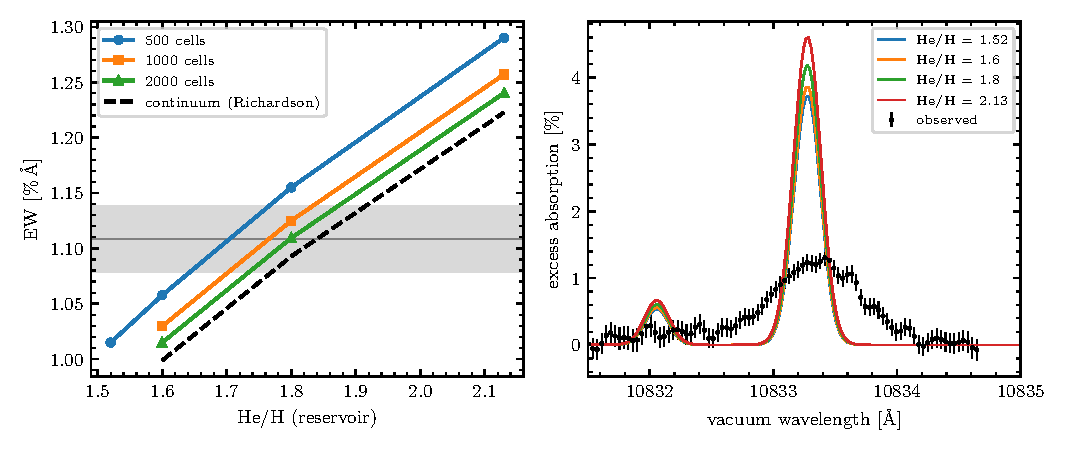
\includegraphics[width=\textwidth]{figures/lhs1140b_kzz1e9_molecular_ew_final.pdf}
\caption{Left: the red-pair EW of the certified molecular states against the
reservoir He/H on 500, 1000 and 2000 cells and in the continuum limit, with
the observed $1.108\pm0.030$~\%\,\AA\ (grey). Right: the unbroadened
500-cell spectra against the released one.}
\label{fig:molewfinal}
\end{figure}

\begin{figure}[htbp]
\centering
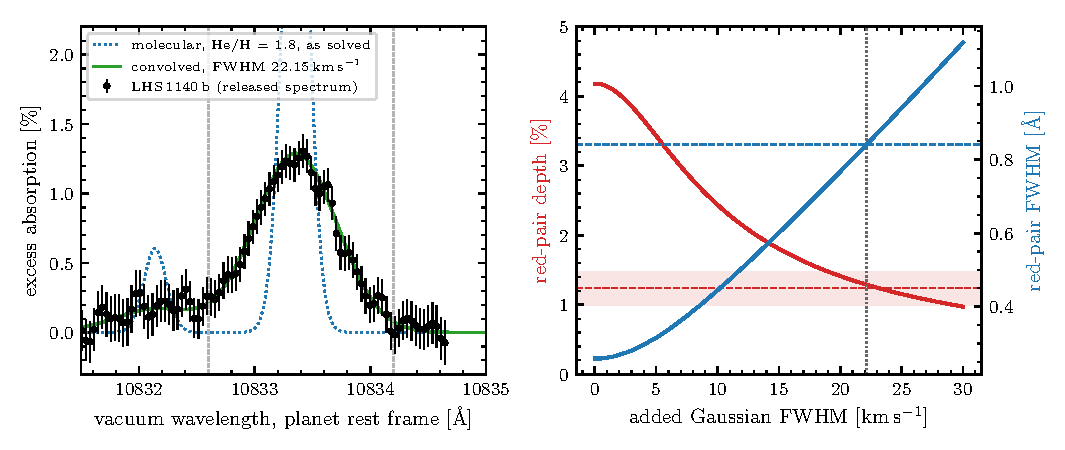
\includegraphics[width=\textwidth]{figures/lhs1140b_kzz1e9_molecular_broadened_final.pdf}
\caption{Left: the molecular He/H~=~1.8 profile as solved (dotted) and
convolved with a 22.15~km\,s$^{-1}$ FWHM Gaussian (solid), against the
released spectrum; both model curves are shifted by the memo's
$v_{\rm wind} = +2.26$~km\,s$^{-1}$ for display (every EW is from the
unshifted arrays), and the dashed verticals mark the EW window. Right: the
red-pair depth (red, left axis) and FWHM (blue, right axis) as the added
Gaussian is scanned; dashed lines are the observed values, the band the
$1\sigma$ interval of the fitted depth, and the dotted vertical the matched
kernel.}
\label{fig:molbroadfinal}
\end{figure}

\begin{figure}[htbp]
\centering
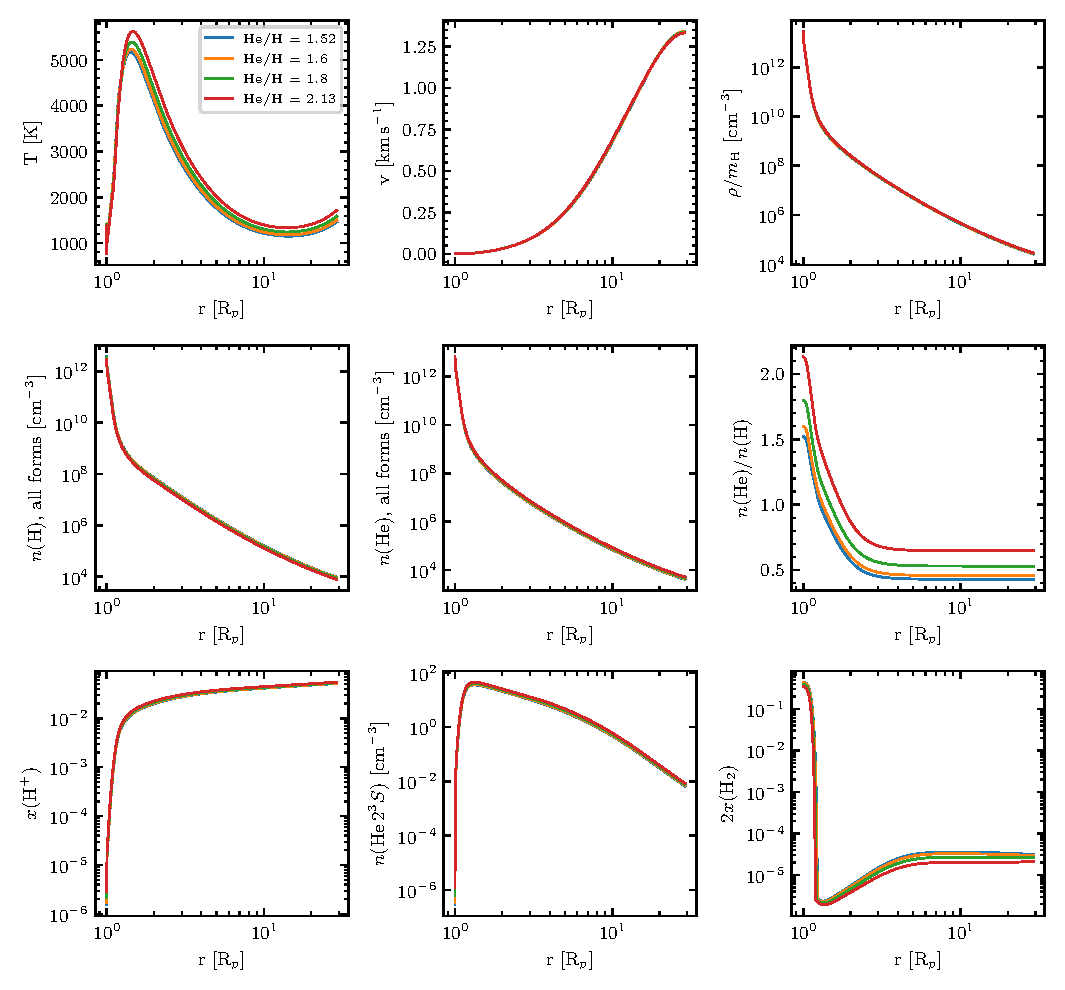
\includegraphics[width=\textwidth]{figures/lhs1140b_kzz1e9_molecular_rungs_final.pdf}
\caption{The certified molecular $K_{zz}=10^{9}$ states He/H~=~1.52 to 2.13
under the corrected atomic physics (advection-corrected profiles):
temperature, velocity, $\rho/m_{\rm H}$, the number densities of all
hydrogen nuclei $n({\rm H})$ and all helium nuclei $n({\rm He})$ (every
ionization stage, level and molecule counted: H~\textsc{i}, H~\textsc{ii},
2\,H$_2$, 2\,H$_2^+$, 3\,H$_3^+$ and HeH$^+$ for hydrogen; He~\textsc{i},
He~\textsc{ii}, He~\textsc{iii} and HeH$^+$ for helium), their ratio
$n({\rm He})/n({\rm H})$, the H~\textsc{ii} fraction, $n({\rm He}\,2^3S)$
and the H$_2$ fraction against radius.}
\label{fig:molrungsfinal}
\end{figure}

\section{What the flux-spread criterion misses, on one certified case}

The question the columns above raise is what a state that meets $du < 10^{-3}$
but fails this code's certification differs from the certified stationary
solution BY. Measured on the atomic \texttt{scalar\_kzz1e9/HeH2.13}, which is certified,
against a state of the same case stopped after one outer pass of the same
route:

\begin{center}
\footnotesize
\begin{tabular}{@{}l l l@{}}
\toprule
 & certified stationary & flux converged, refused\\
\midrule
$du$, the run's own gate & 2.46E-11 & 1.83E-12\\
$\lVert R\rVert$, re-evaluated & 1.61E-08 & 4.97E-08\\
the three hydrodynamic rows & within & within\\
elemental transport He/H, $r \ge 1.2$ & within & 5.21E-05 above 1.0E-05 at $r = 1.695$\\
verdict & CERTIFIED & NOT CERTIFIED, one entry\\
\bottomrule
\end{tabular}
\end{center}

\noindent
Both clear the flux-spread criterion by four to eight decades and ONE row
separates them. The two states differ by at most 1.9 per cent in any profile,
and the difference sits in the composition and the temperature of the layer
the He~I 10830 line forms in (the metastable column's median radius is
6.4~$R_p$, its 5 to 95 per cent range 1.7 to 16.7~$R_p$), not in
$\rho v r^2$, which agrees to 0.055 per cent everywhere. That is why the
flux-spread criterion is blind to it.

It reaches a measured quantity. With the catalog's own selection the He~I
10830 red-pair equivalent width moves from 1.374869 to 1.356745~\%\,\AA, a
change of 1.32 per cent, and the red depth by 1.11 per cent, while
$\log_{10}\dot{M}$ is 7.87 for both at the two decimals the code prints. For
scale, the He/H rungs of this group stand 0.178~\%\,\AA\ apart in the
equivalent width, so the shift is a tenth of the spacing the ladder measures
a composition with.

Against the measurement it is smaller still. The observed red-pair equivalent
width is $1.108 \pm 0.029$~\%\,\AA, integrated from the spectrum Cherubim
et al.\ (2026) released, with the error of the same estimator under
independent sample errors (our number, not the paper's; the tables and figures
of this document were drawn with $\pm 0.030$, the error before the estimator
was given its own trapezoidal weights on 2026-09-29), and the two states
differ by 0.018~\%\,\AA, which is 0.62 of one standard deviation. For a comparison with the data the
two states are the same model: the refused one would be read as the same
answer. What the certification buys is not a different observable but the
statement that the state solves the elemental transport equation everywhere,
which is what lets a later measurement, or a ladder that resolves 0.178
\%\,\AA\ in composition, rest on it.

\begin{figure}[htbp]
\centering
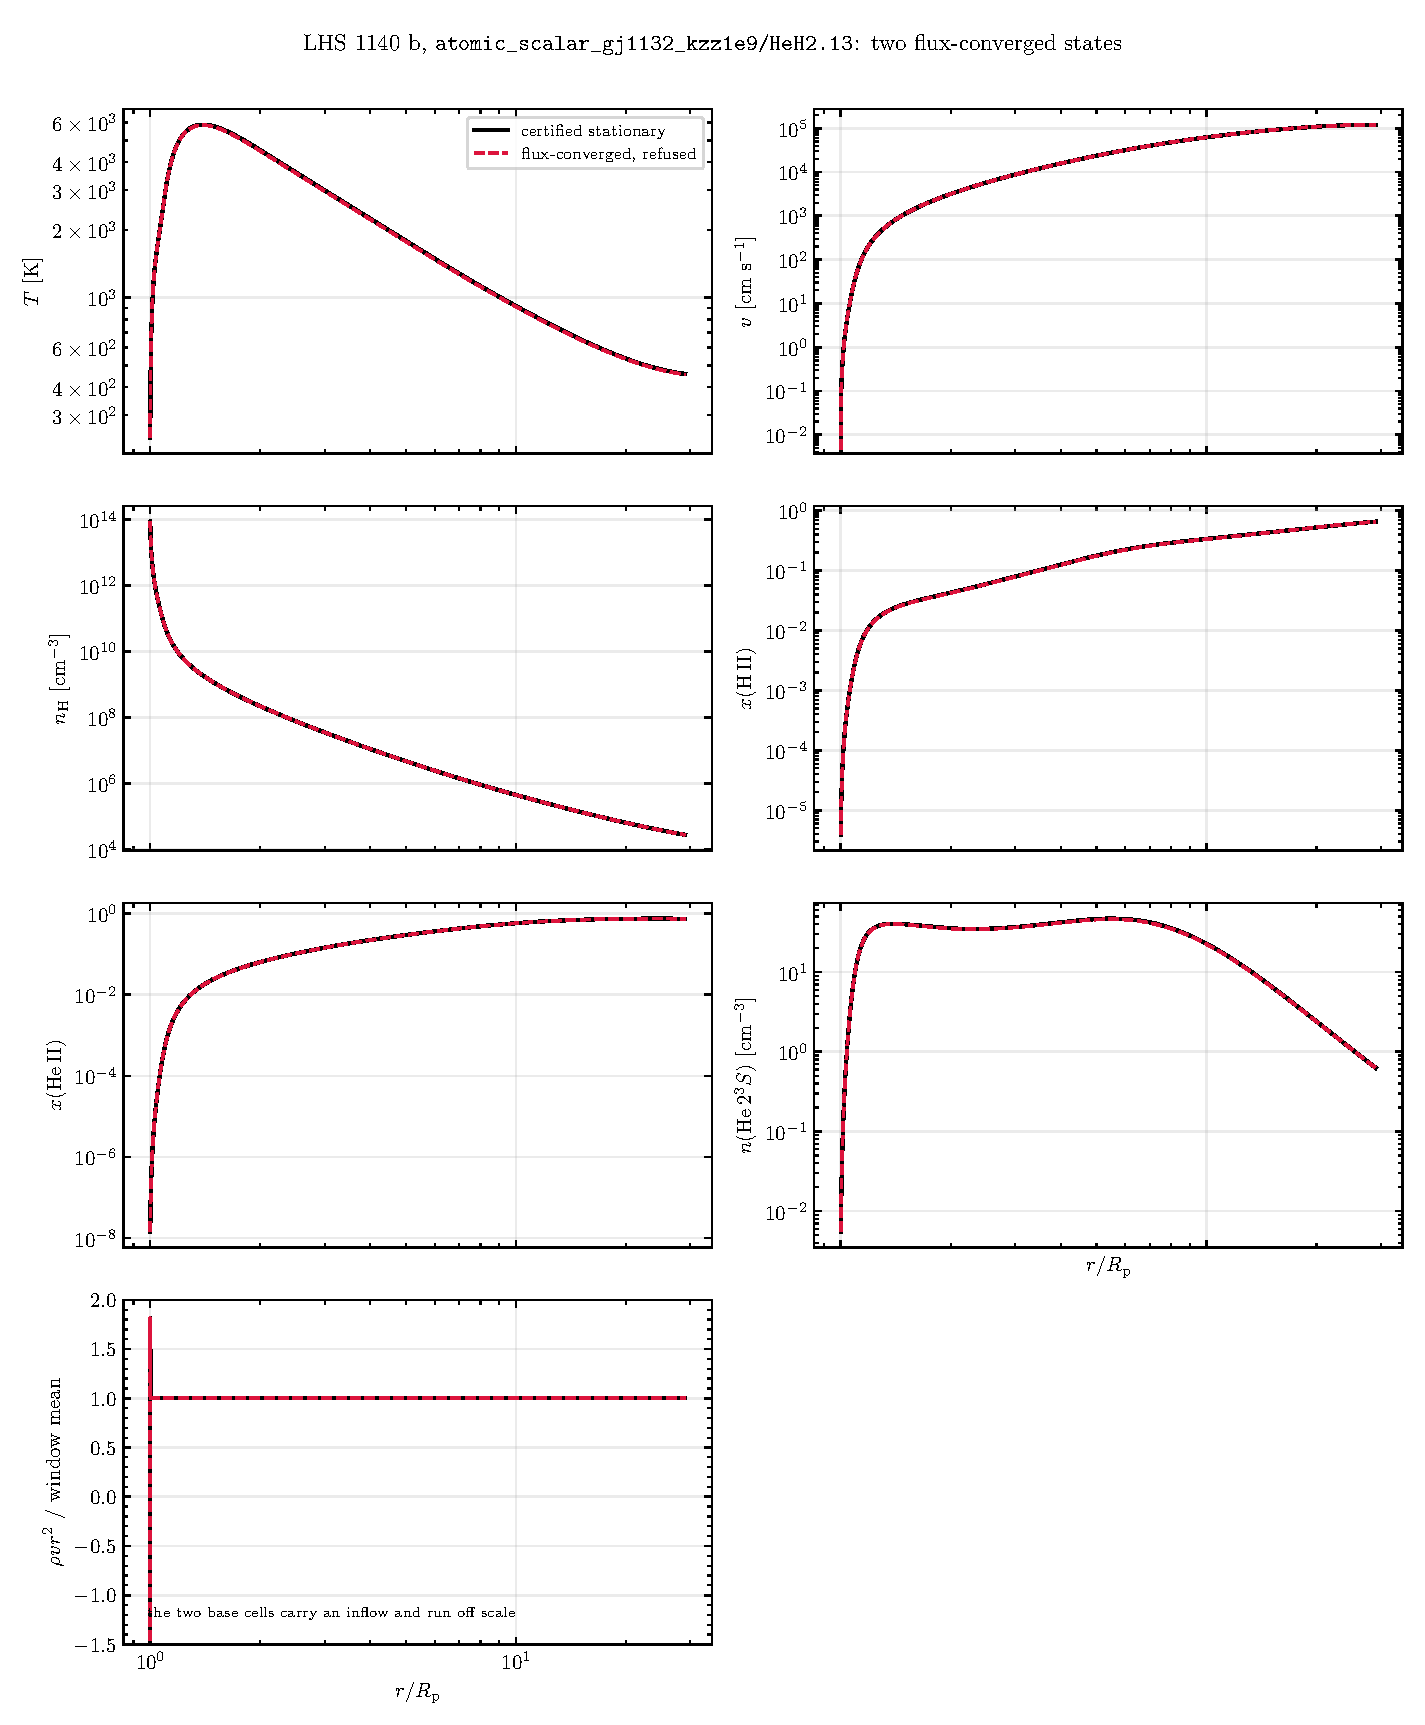
\includegraphics[width=\textwidth]{figures/du_stop_vs_stationary_profiles.pdf}
\caption{The certified stationary solution and the flux-converged refused
state of the atomic \texttt{scalar\_kzz1e9/HeH2.13}, as functions of radius.
The last panel is the number density of all helium nuclei, He~\textsc{i} +
He~\textsc{ii} + He~\textsc{iii}, independent of ionization and level.}
\end{figure}

\begin{figure}[htbp]
\centering
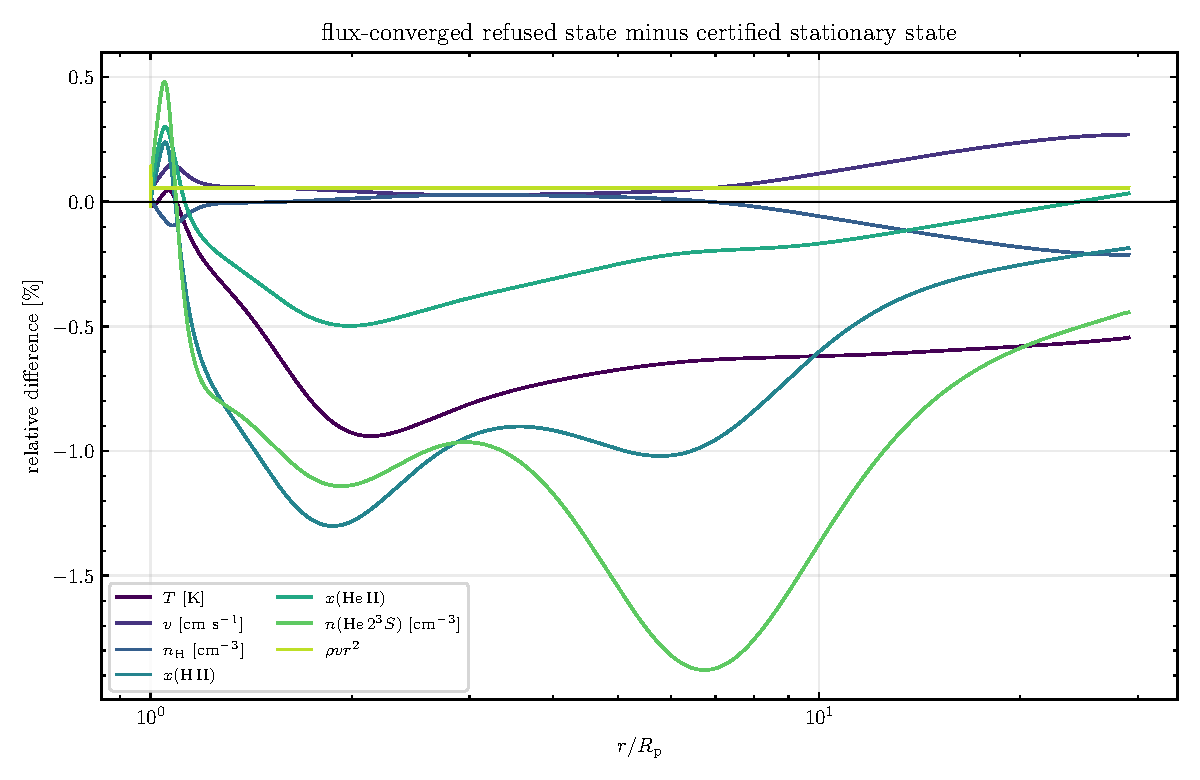
\includegraphics[width=\textwidth]{figures/du_stop_vs_stationary_differences.pdf}
\caption{The same two states, as the relative difference of each quantity.
The largest are the temperature at $r = 2.13\,R_p$ ($-0.94$ per cent),
$x(\mathrm{H\,II})$ at 1.87 ($-1.30$) and $n(\mathrm{He}\,2^3S)$ at 6.74
($-1.88$).}
\end{figure}

\begin{figure}[htbp]
\centering
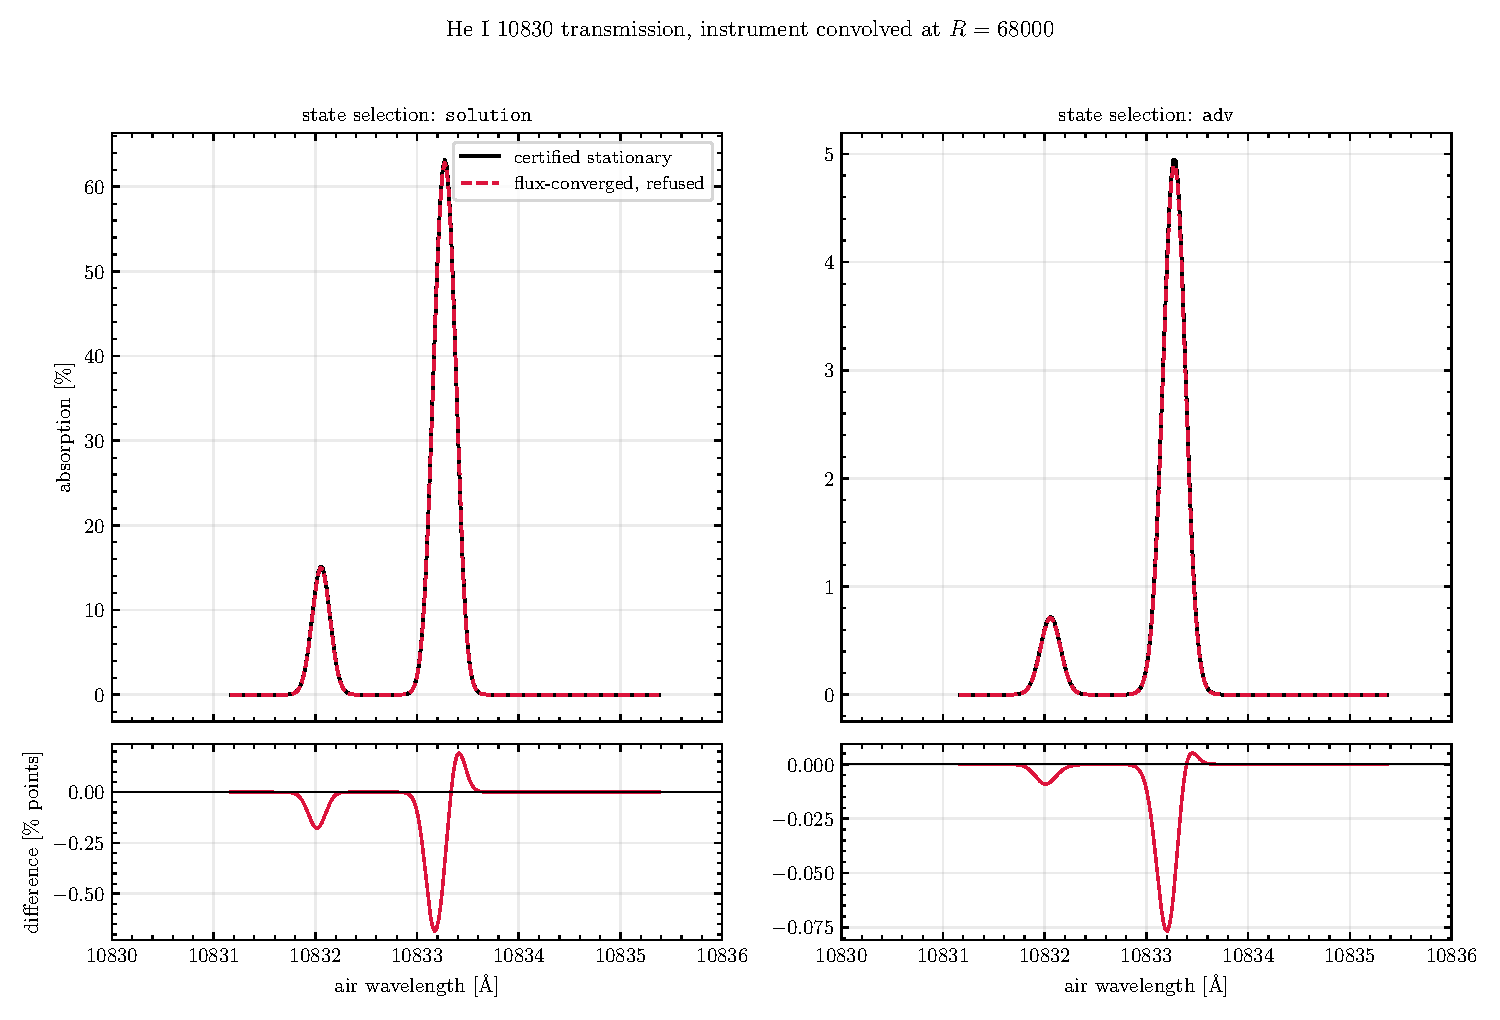
\includegraphics[width=0.85\textwidth]{figures/du_stop_vs_stationary_he10830.pdf}
\caption{The He~I 10830 transmission of the two states.}
\end{figure}

\end{document}
